\chapter{Resultados}
\label{chap:resultados}

Em vista dos procedimentos teóricos aliados a uma solução computacional, obteve-se os seguintes resultados:
\begin{itemize}
    \item resposta em frequência;
    \item sugestão de notas;
    \item sugestão de acordes;
    \item detecção de transições rítmicas;
    \item implementação da transformada wavelets;
    \item transcrição de notas ao longo do tempo;
    \item extração da tonalidade do áudio;
    \item transcrição automática de acordes ao longo do tempo.
\end{itemize}

% Comentar cada item e o fundamento teórico por trás de cada um

\section{Resposta em Frequência e Sugestões de Notas e Acordes}

Para a demonstração de tais resultados foram feitos experimentos com todas as possibilidades de reconhecimento de acordes proporcionados pelo sistema. Todavia serão detalhados e comentados somente 4 pois para os outros equivalem as mesmas considerações. O resumo dos resultados dos outros acordes estará presente na tabela que se segue logo após. Esses experimentos foram feitos levando em consideração pré-condições e pós-condições.
\newpage

\subsection{Pré-condições dos Experimentos}
\label{sec:precondicoes}

No que tange às pré-condições foram levados em conta:
\begin{itemize}
    \item teclado yamaha E413 com som de piano para a execução dos acordes;
    \item somente tríades (3 notas) tocadas;
    \item o software Audacity \footnote{http://www.audacity.sourceforge.net} foi utilizado para gravação;
    \item o microfone convencional interno do $notebook$ foi utilizado para aquisição dos sinais de áudio;
    \item o ruído de fundo estava com uma grandeza por volta de 45 db;
    \item a taxa de amostragem do sinal foi configurada em 44100 Hz;
    \item gravação do áudio no formato de arquivo .wav em codificação 16 pcm.
\end{itemize}

\newpage
As tríades de acordes foram executadas com base na nota central $C4$ que possui o valor de aproximadamente 261,6 Hz. A figura \ref{fig:teclado} ilustra as regiões e limites usados \cite{teclado}:

\begin{figure}[h]
	\centering
		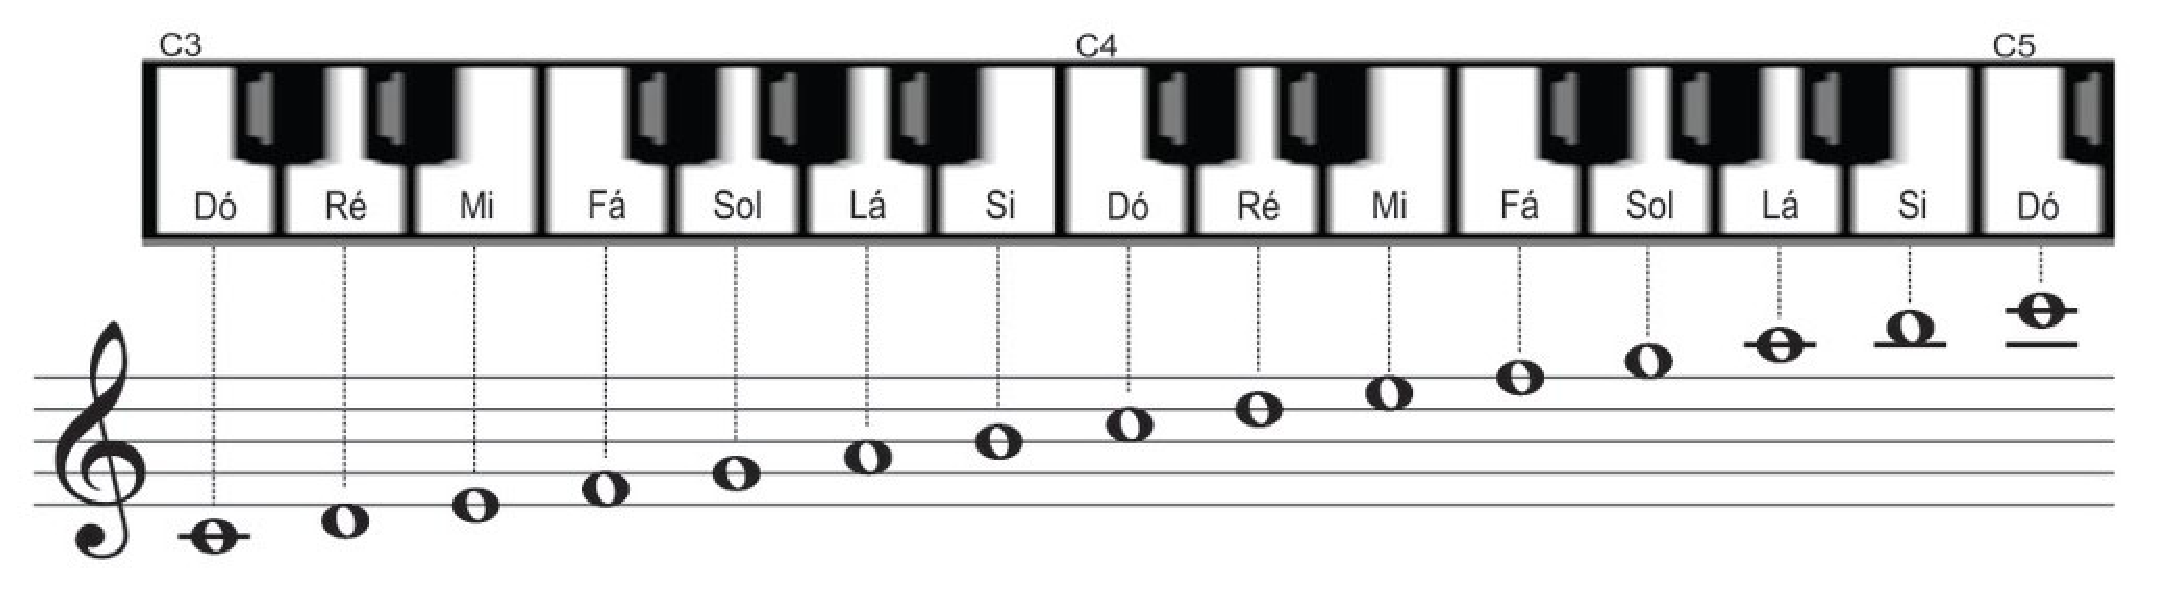
\includegraphics[keepaspectratio=true,scale=0.4]{figuras/teclado-tcc1.eps}
	\caption{Teclado ilustrativo para execução dos acordes}
  \label{fig:teclado}
\end{figure}

O processo de execução do experimento foi dividido em 4 etapas. A primeira relativa a gravação do acorde tocado no teclado via microfone convencional interno do $notebook$. A segunda é a exportação do som no formato de arquivo .wav pelo software audacity. A terceira etapa é a introdução do arquivo na entrada do sistema de detecção de acordes. A última atividade é a classificação do arquivo digital num acorde. A figura \ref{fig:processo} ilustra o processo esquematizado.

\begin{figure}[h]
	\centering
		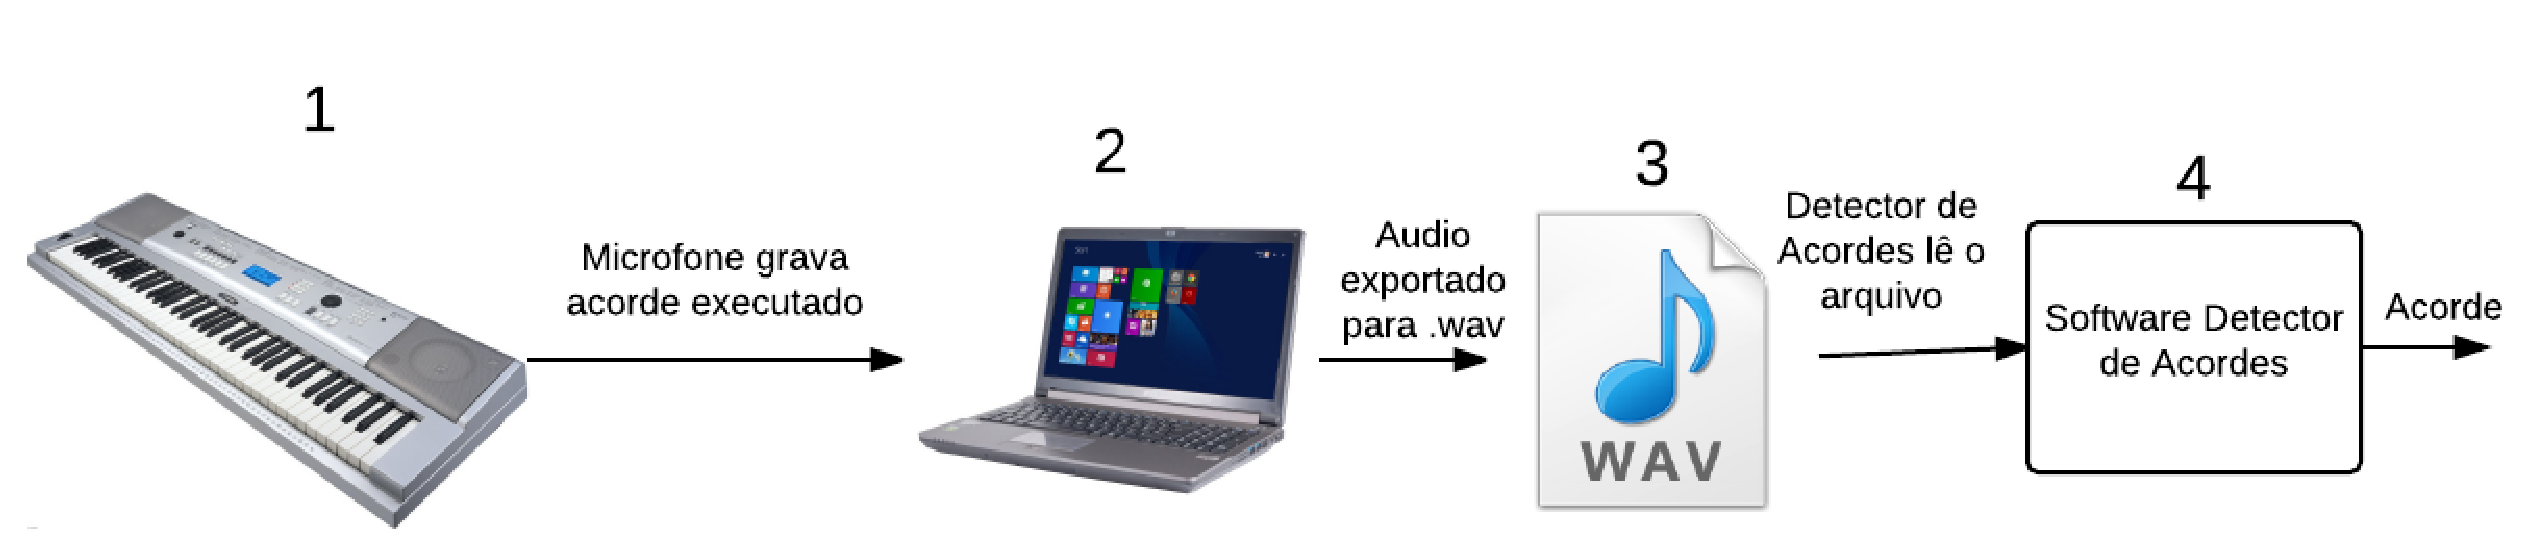
\includegraphics[keepaspectratio=true,scale=0.35]{figuras/processo_experimento.eps}
	\caption{Processo ilustrativo da execução dos experimentos}
  \label{fig:processo}
\end{figure}

\newpage
\subsection{Experimento 1 - Acorde $CM$}
\label{sec:experimento1}

Nesse experimento foi tocado a tríade $Dó$ (baixo e tônica), $Mi$ e $Sol$ equivalente ao acorde $CM$. A tríade foi tocada ao mesmo tempo e com a mesma força para todas as notas.

Segue os gráficos resultantes:

\begin{figure}[h]
	\centering
		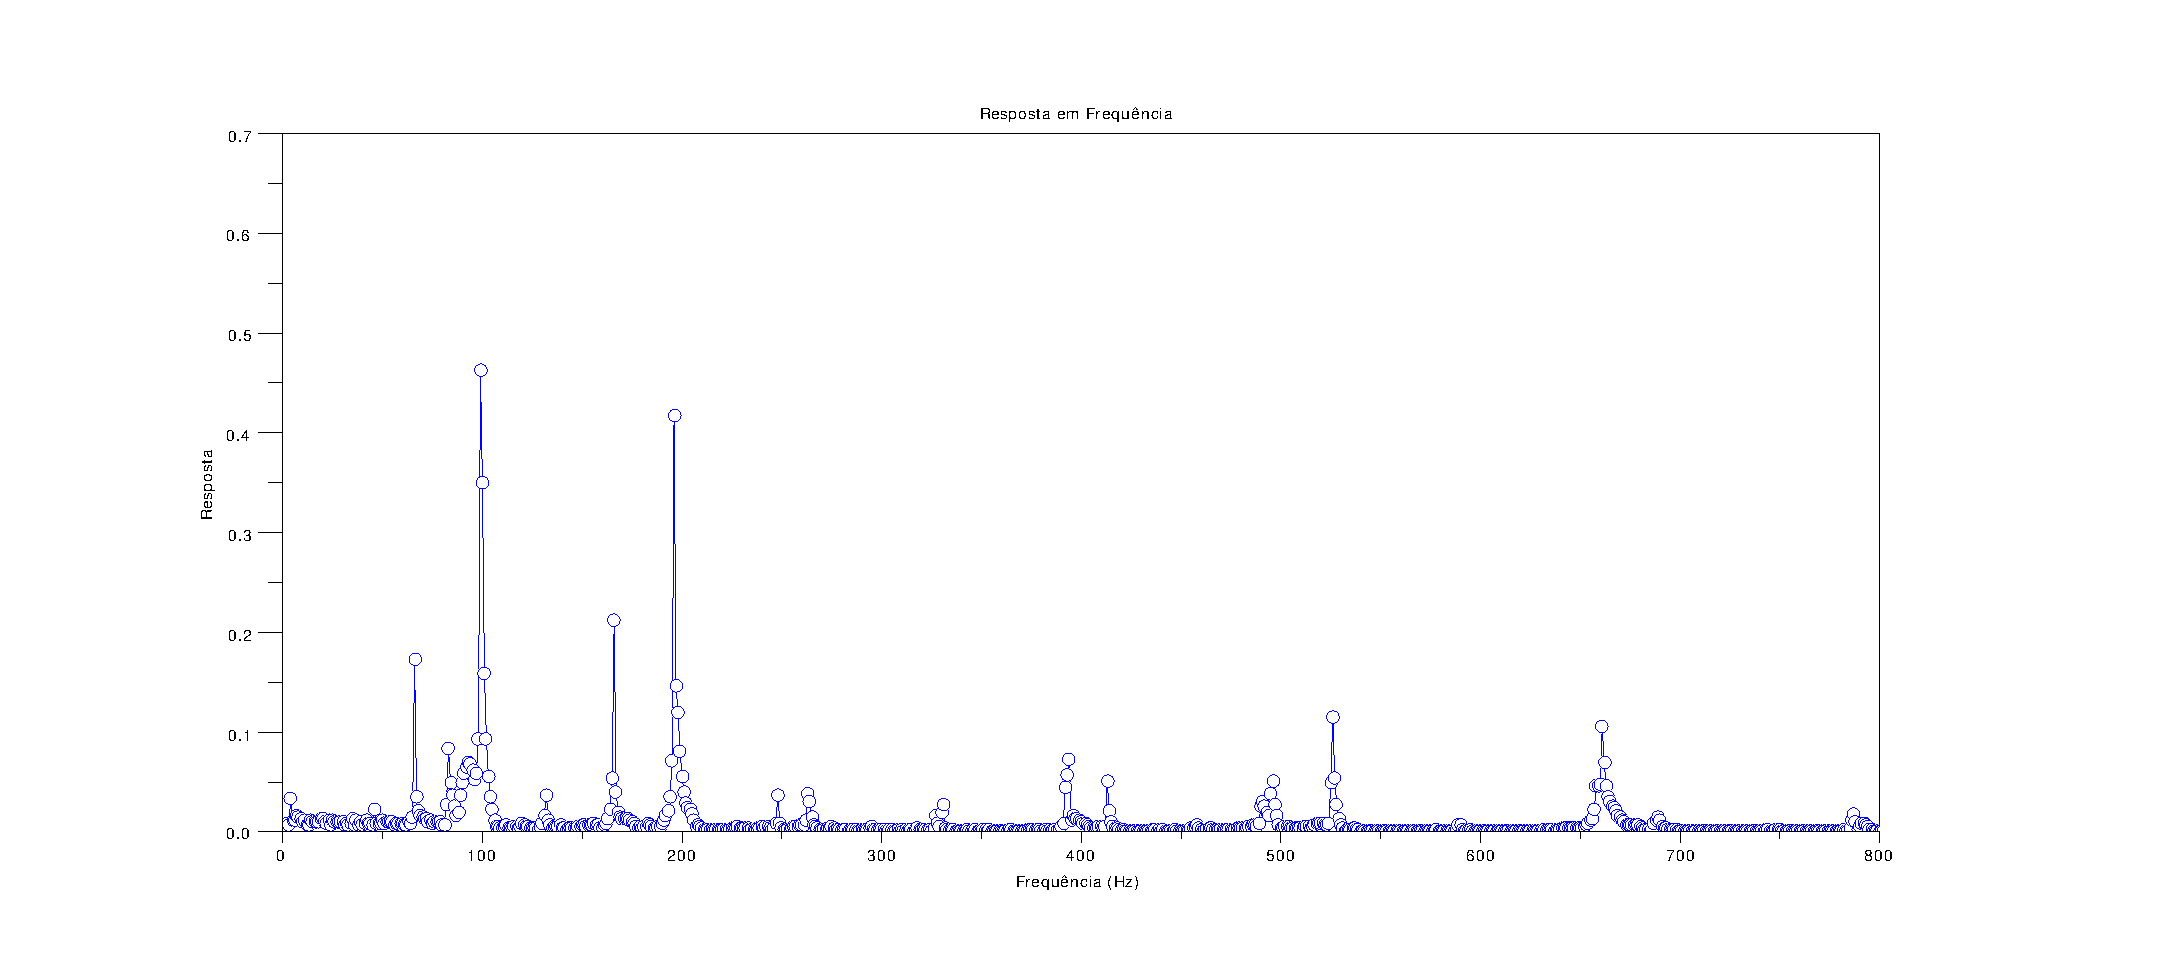
\includegraphics[keepaspectratio=true,scale=0.49]{figuras/CM/fft_cm.eps}
	\caption{Gráfico da resposta em frequência para a gravação do acorde $CM$}
  \label{fig:espectro_CM}
\end{figure}

\begin{figure}[h]
	\centering
		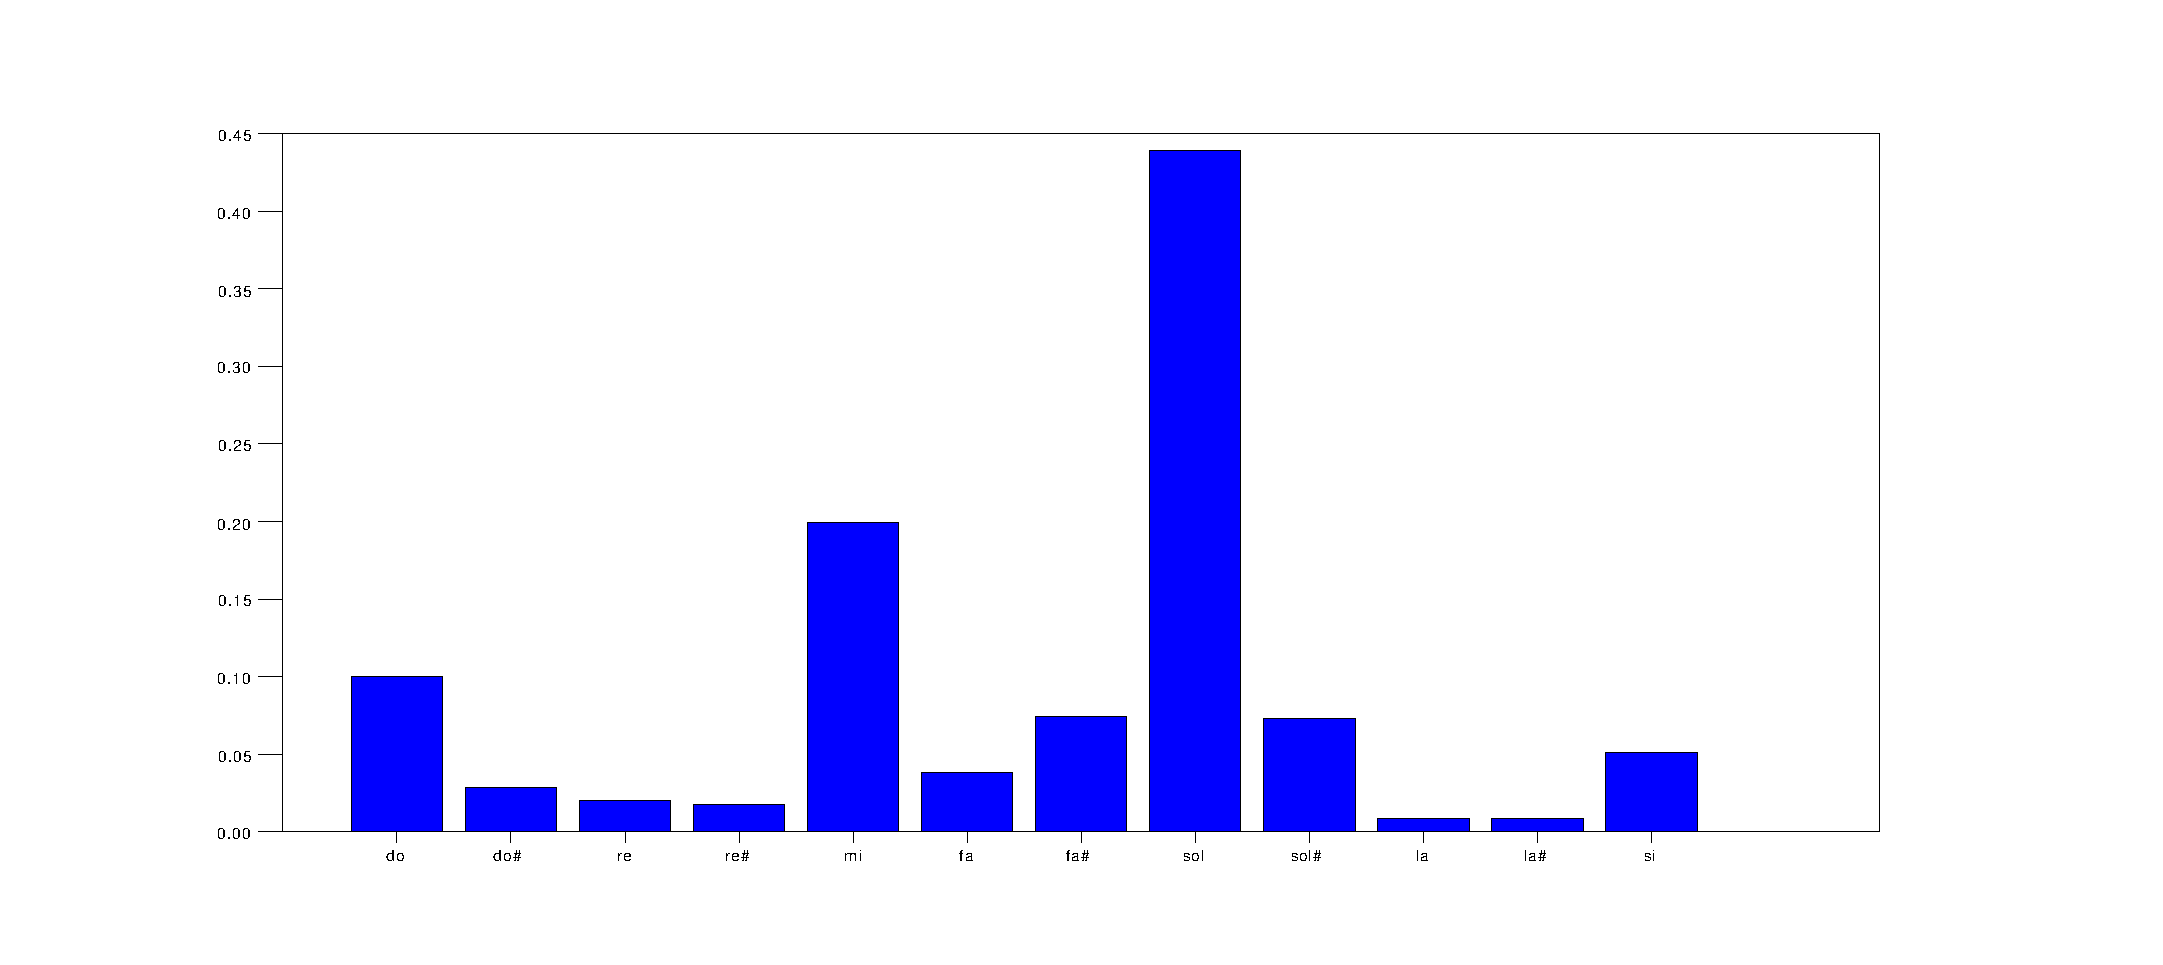
\includegraphics[keepaspectratio=true,scale=0.49]{figuras/CM/notas_cm.eps}
	\caption{Gráfico de sugestão de notas para a gravação do acorde $CM$}
  \label{fig:notas_CM}
\end{figure}

\begin{figure}[h]
	\centering
		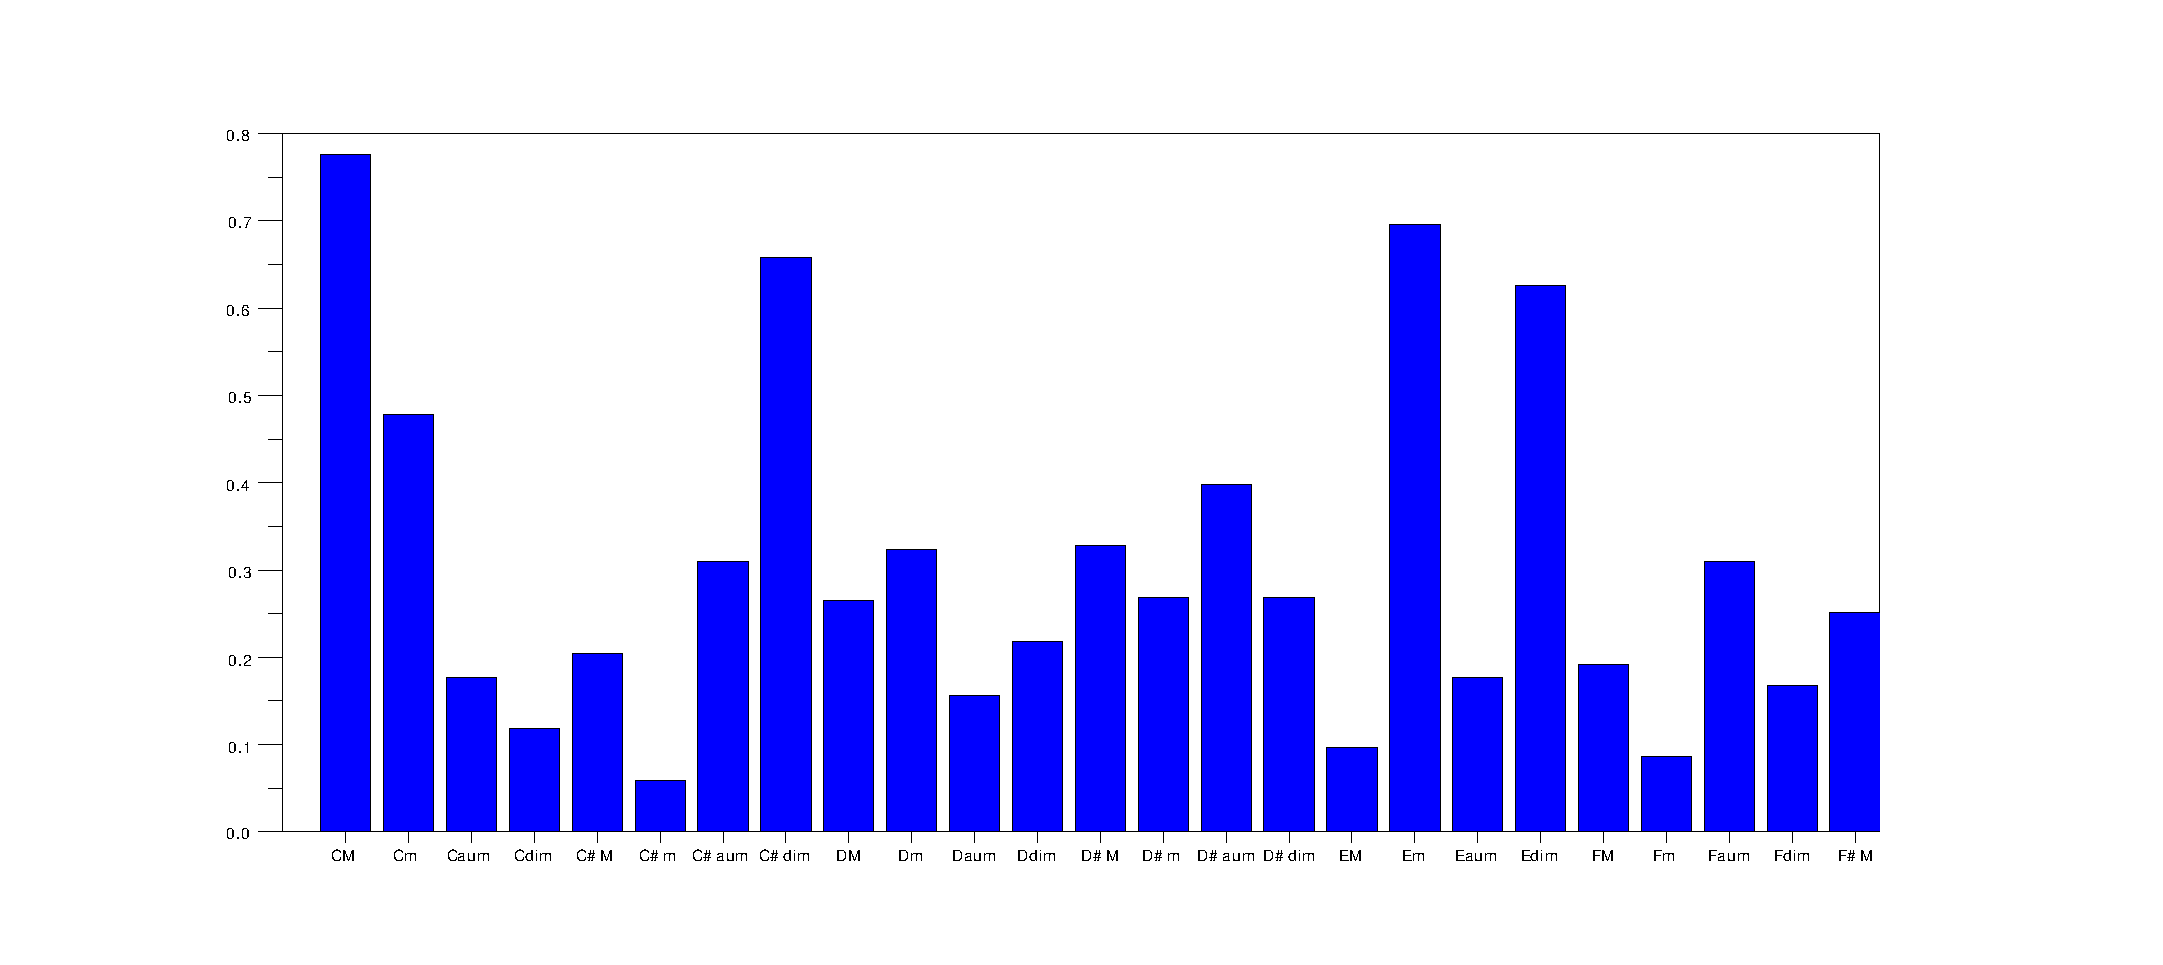
\includegraphics[keepaspectratio=true,scale=0.45]{figuras/CM/acordes_1_cm.eps}
		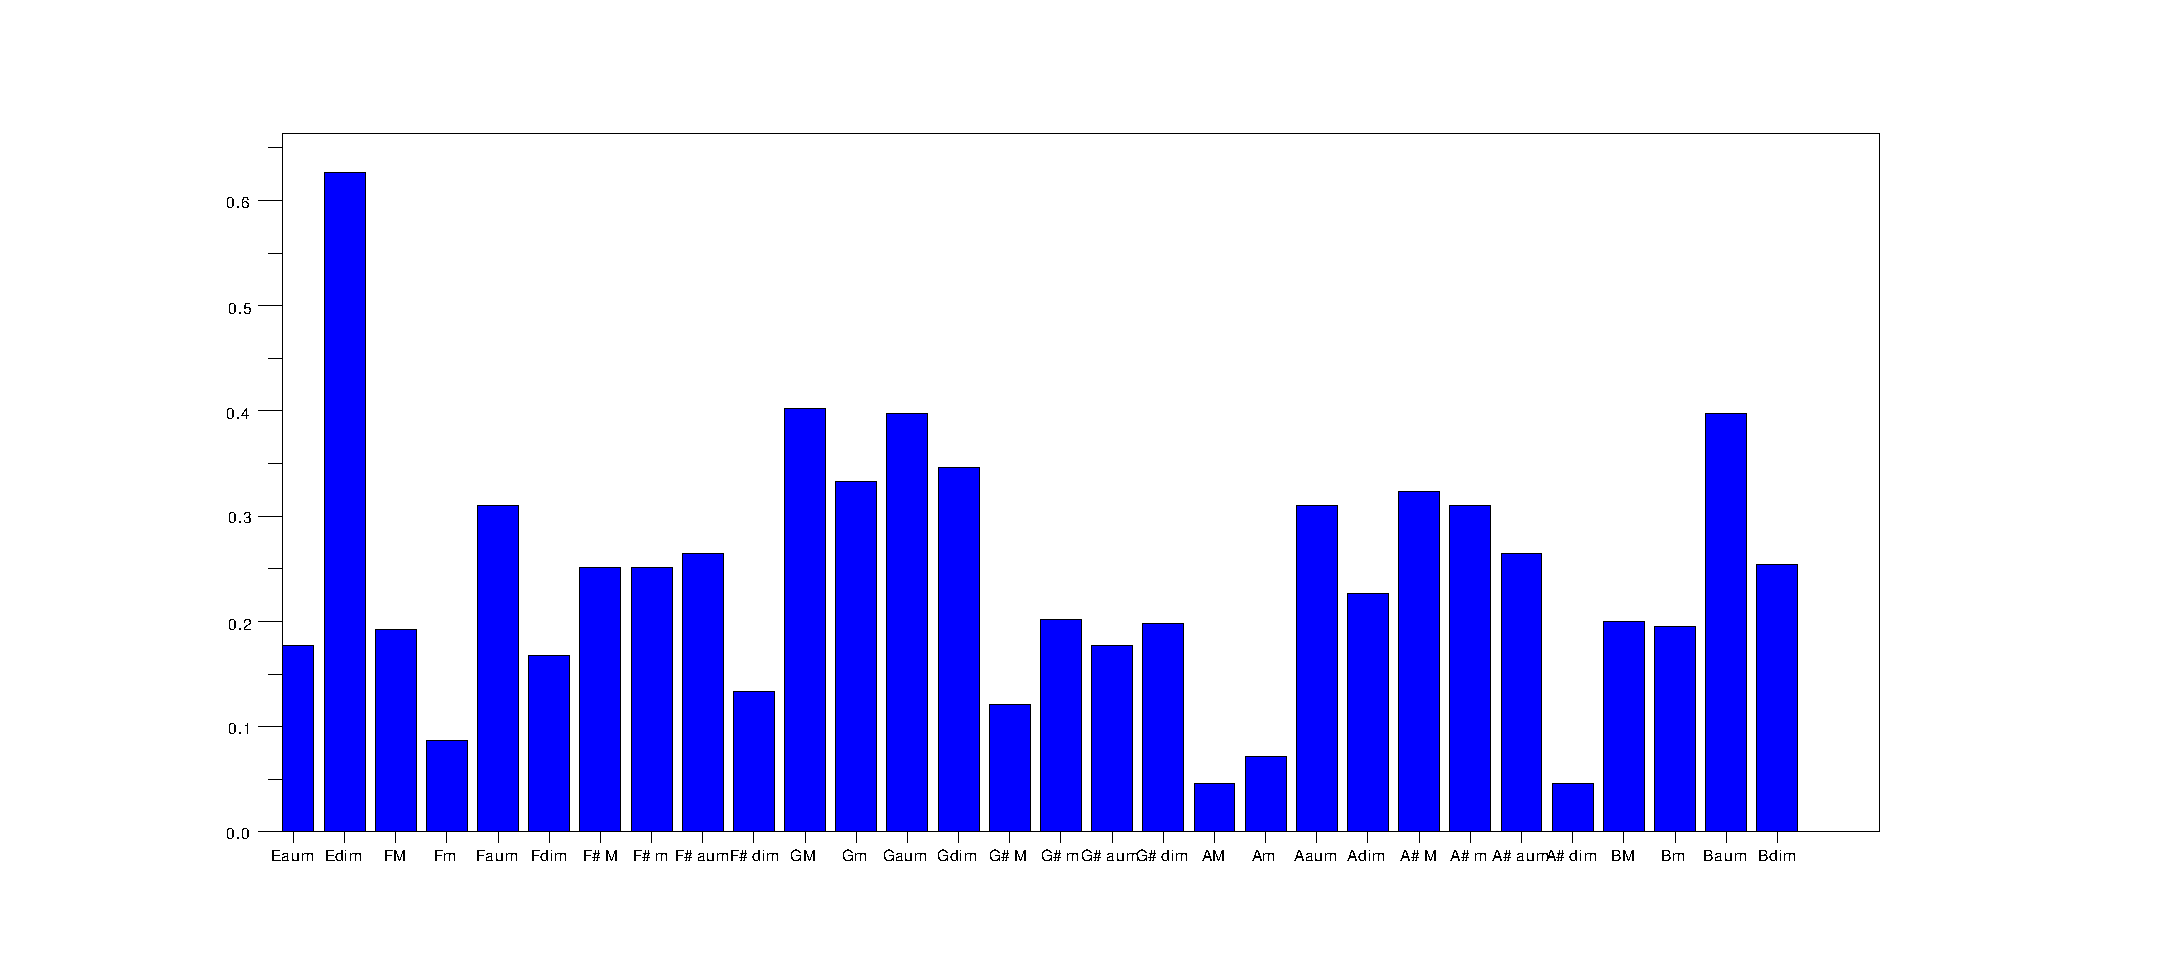
\includegraphics[keepaspectratio=true,scale=0.45]{figuras/CM/acordes_2_cm.eps}
	\caption{Gráficos de sugestão de acordes a gravação do acorde $CM$}
  \label{fig:acordes_CM}
\end{figure}
\newpage
Do resultado da primeira camada de processamento é gerado o gráfico da figura \ref{fig:espectro_CM}. Esse gráfico diz respeito a natureza da composição do sinal em senoides em termos de transformada de fourier. O primeiro pico, no valor de 294 Hz, é relativo a nota $Dó$. O segundo pico, no valor de 371 Hz, é relativo a nota $Mi$. O terceiro pico, no valor de 441 Hz, é relativo a nota $Sol$. Os picos seguintes são relativos aos harmônicos dessas três notas.

Do resultado da segunda camada de processamento é gerado gráfico da figura \ref{fig:notas_CM}. É possível perceber nele que as notas $Dó$, $Mi$ e $Sol$ são as que mais possuem energia ou, no ponto de vista de sugestão, as mais sugeridas. De certa forma um dos fatores que contribuiram das notas $Dó$ e $Sol$ ser de maiores energias foi devido a presença dos harmônicos.

Do resultado da terceira camada de processamento são gerados os gráficos da figura \ref{fig:acordes_CM}. Essa camada é relativa ao resultados das sugestões de acordes musicais. É perceptível ver a presença da alta sugestão do acorde $CM$.

\subsection{Experimento 2 - Acorde $Dm$}
\label{sec:experimento2}

Nesse experimento foi tocado a tríade $Ré$ (baixo e tônica), $Fá$ e $Lá$ equivalente ao acorde $Dm$. A tríade foi tocada ao mesmo tempo e com a mesma força para todas as notas.

Segue os gráficos resultantes:

\begin{figure}[h]
	\centering
		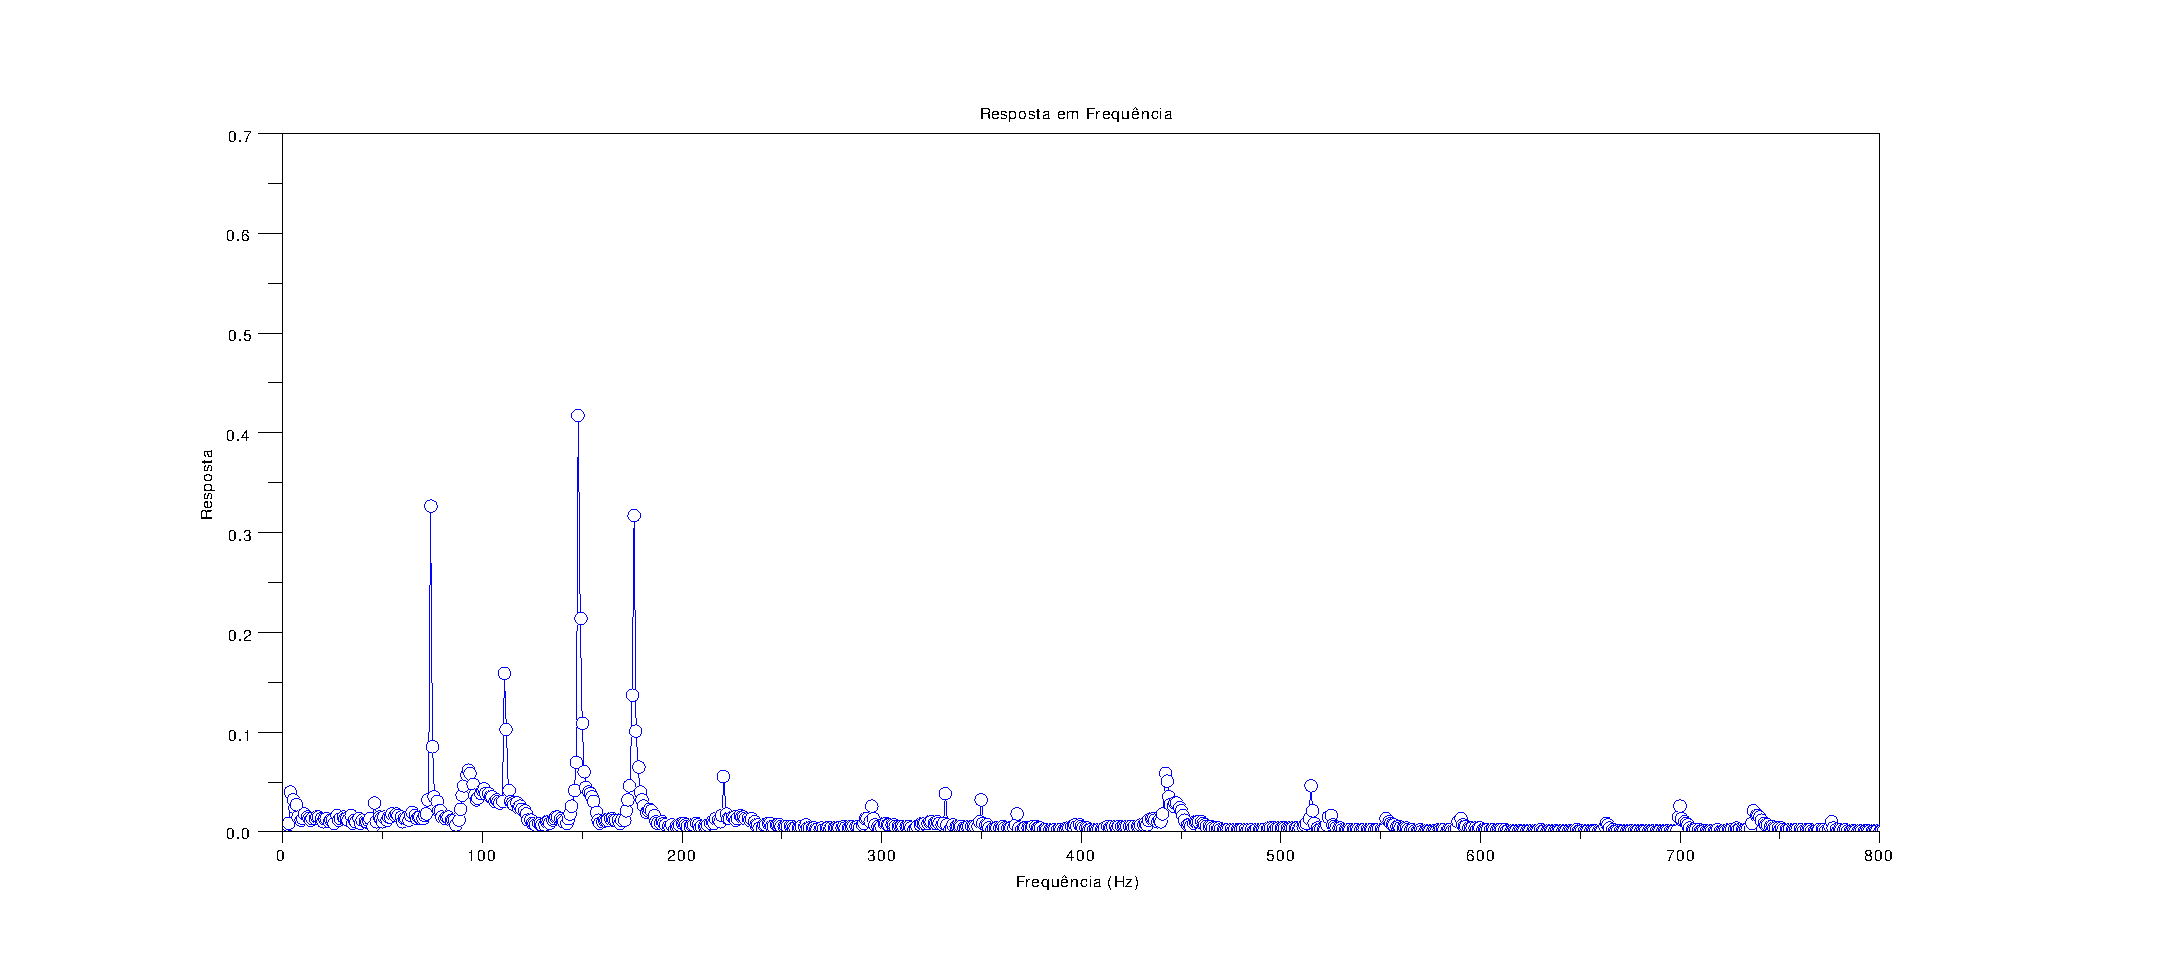
\includegraphics[keepaspectratio=true,scale=0.49]{figuras/Dm/fft_Dm.eps}
	\caption{Gráfico da resposta em frequência para a gravação do acorde $Dm$}
  \label{fig:espectro_Dm}
\end{figure}

\begin{figure}[h]
	\centering
		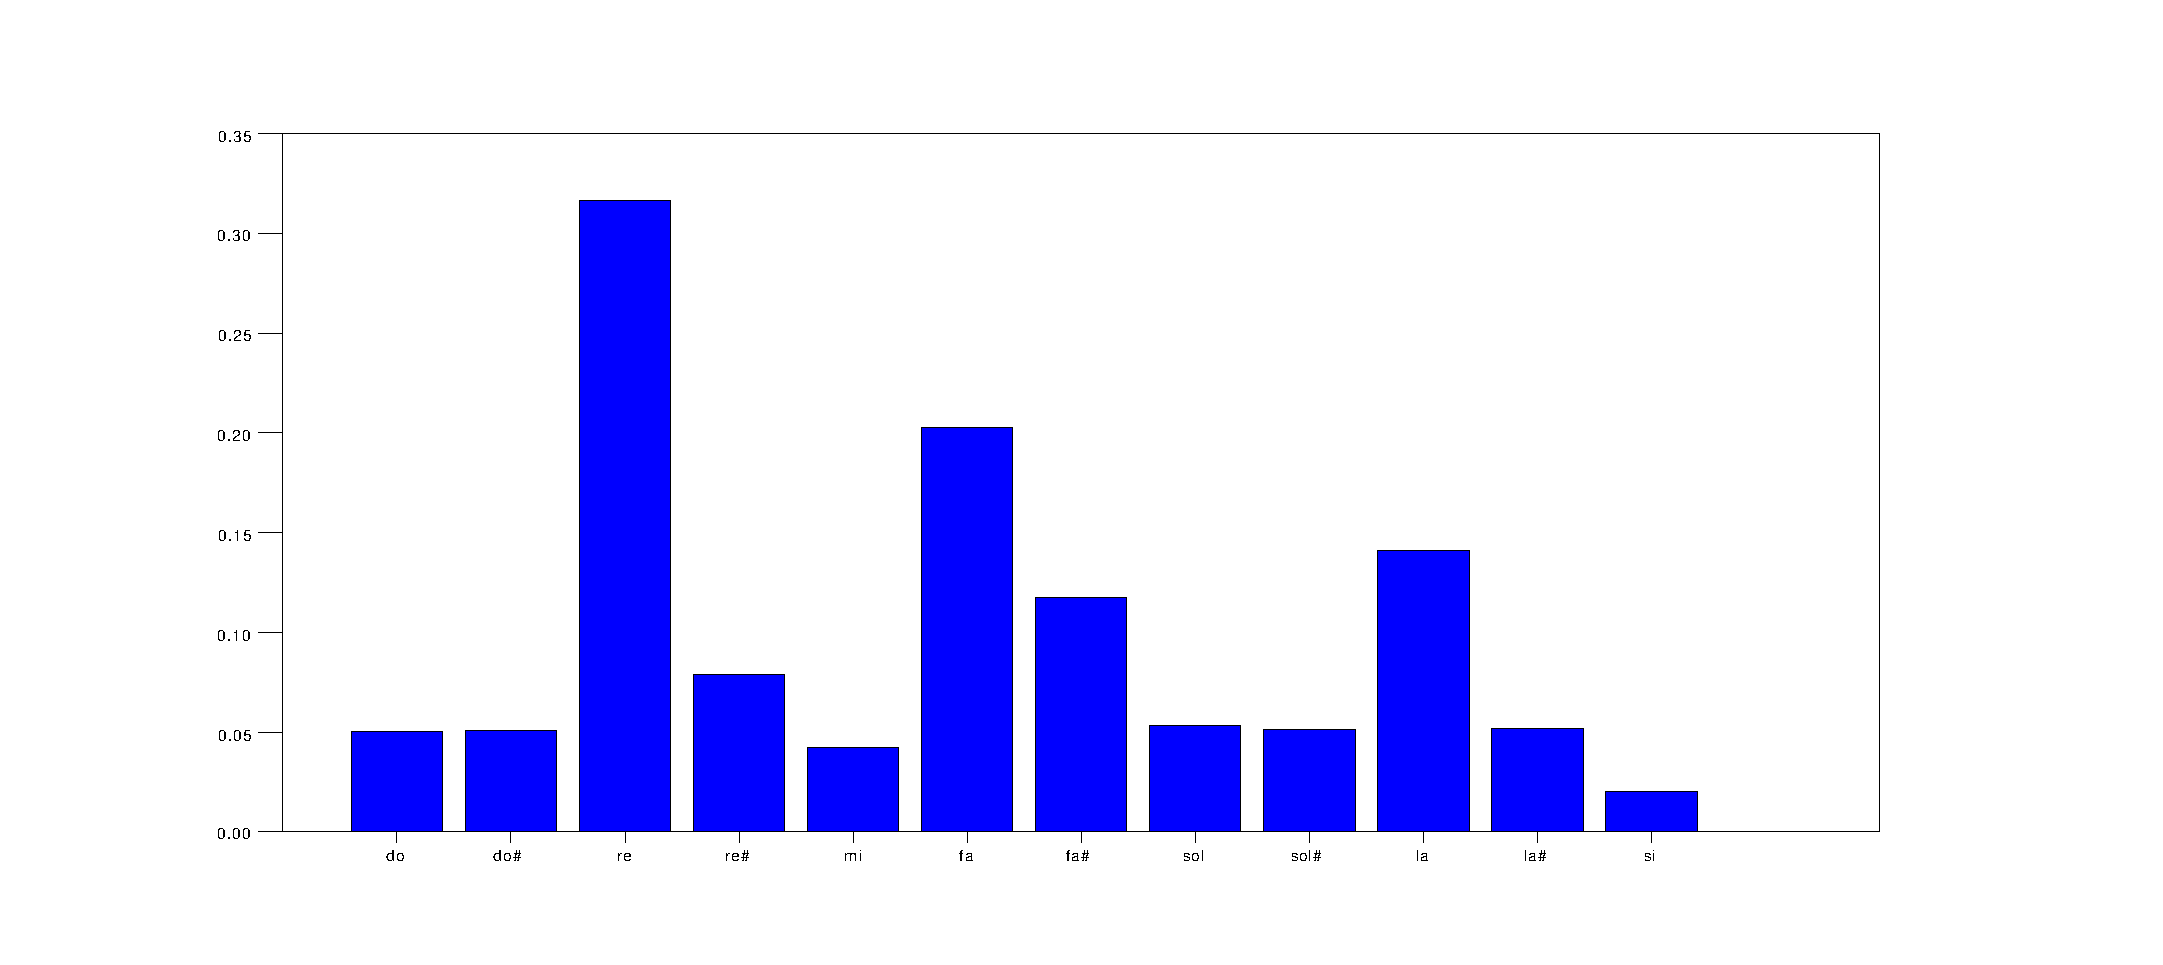
\includegraphics[keepaspectratio=true,scale=0.49]{figuras/Dm/notas_Dm.eps}
	\caption{Gráfico de sugestão de notas para a gravação do acorde $Dm$}
  \label{fig:notas_Dm}
\end{figure}

\begin{figure}[h]
	\centering
		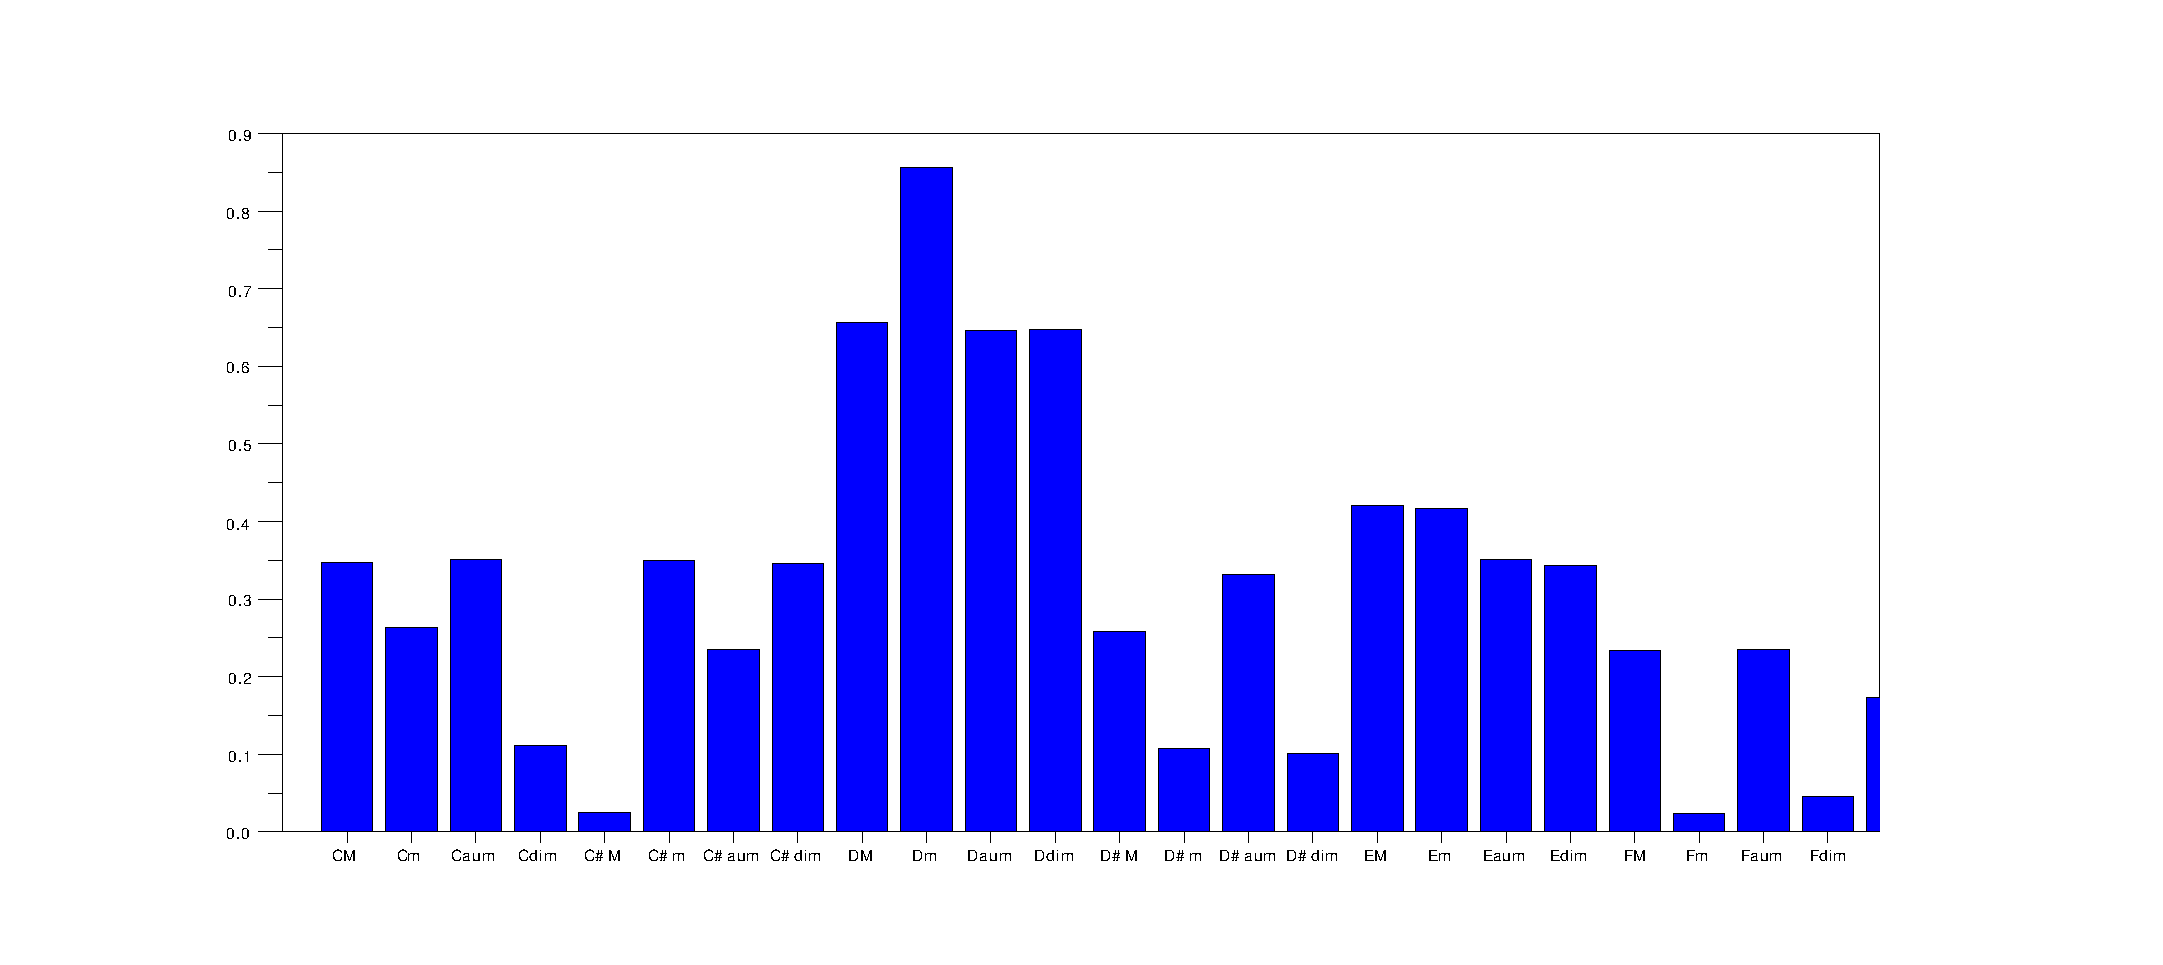
\includegraphics[keepaspectratio=true,scale=0.49]{figuras/Dm/acordes_1_Dm.eps}
		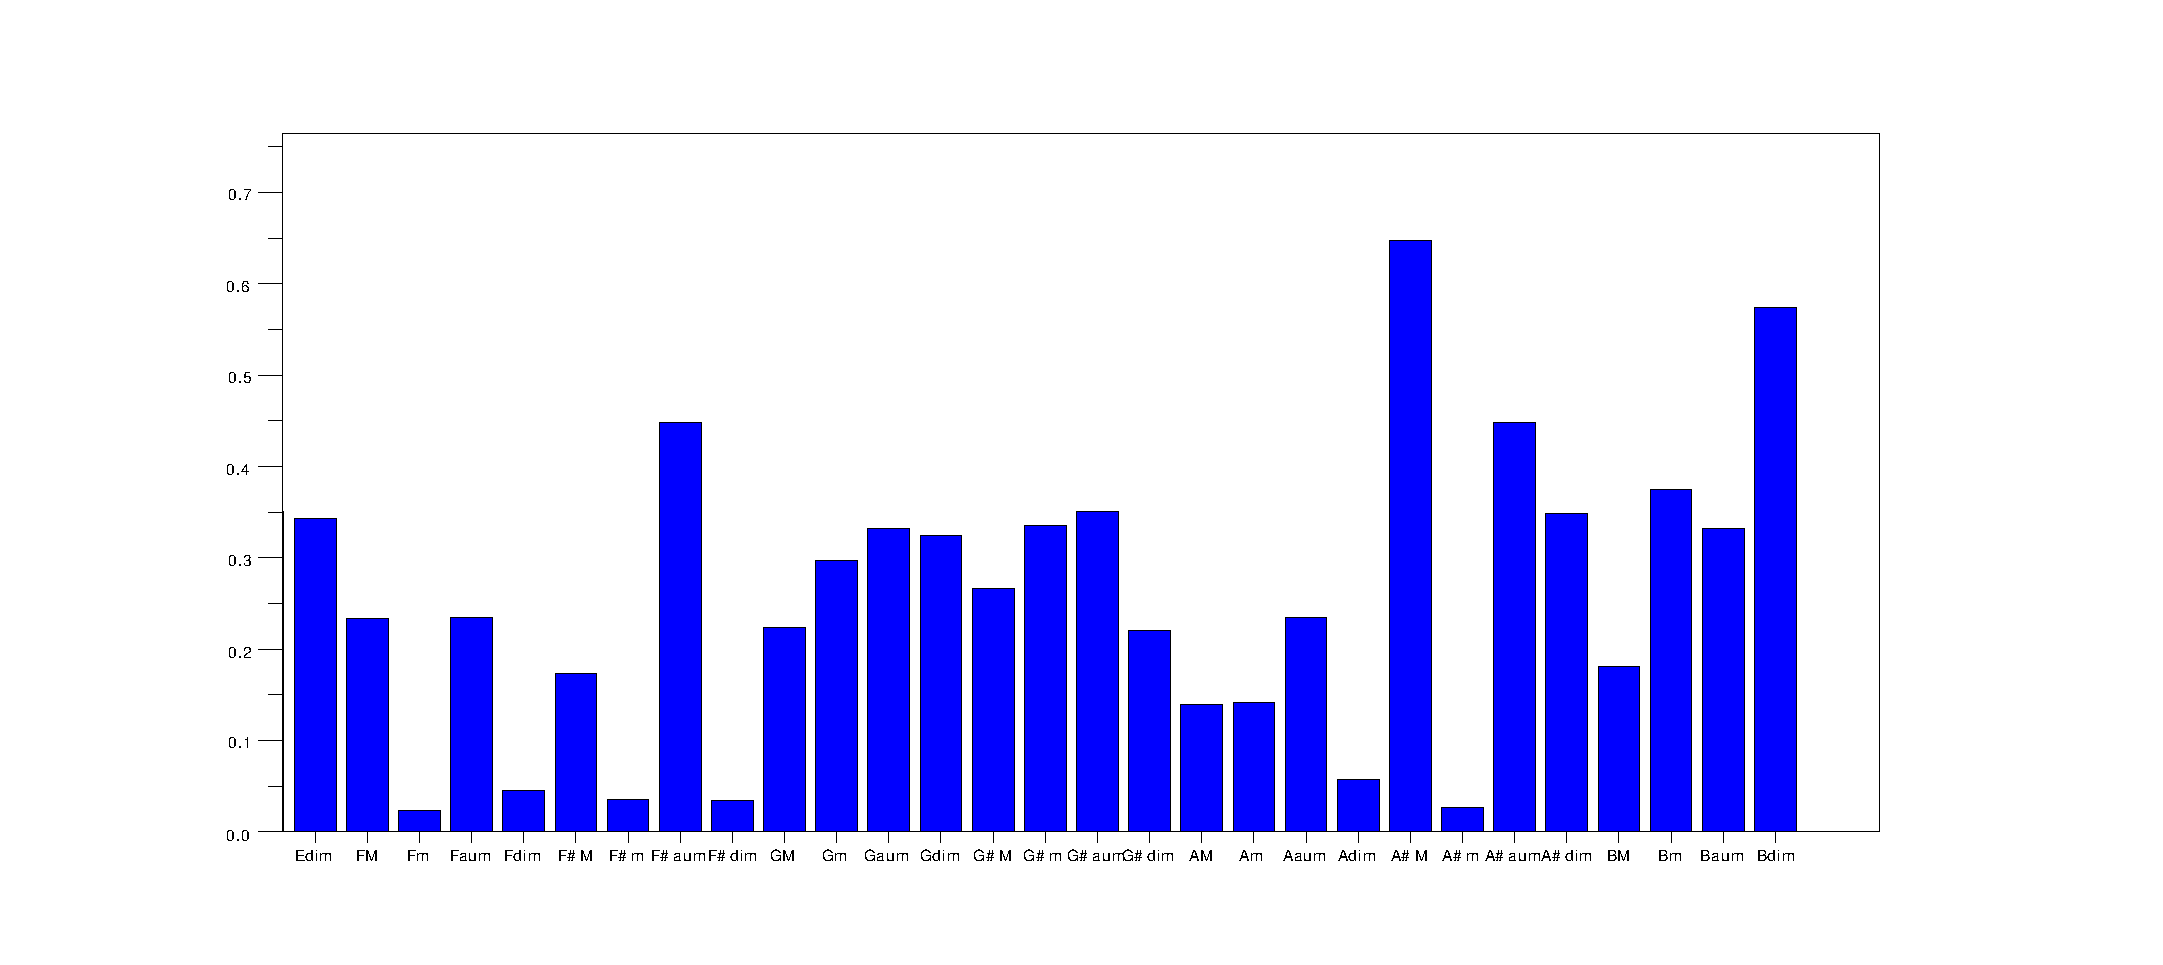
\includegraphics[keepaspectratio=true,scale=0.49]{figuras/Dm/acordes_2_Dm.eps}
	\caption{Gráficos de sugestão de acordes a gravação do acorde $Dm$}
  \label{fig:acordes_Dm}
\end{figure}
\newpage

Do resultado da primeira camada de processamento é gerado o gráfico da figura \ref{fig:espectro_Dm}. Esse gráfico diz respeito a natureza da composição do sinal em senoides em termos de transformada de fourier. O primeiro pico, no valor de 294 Hz, é relativo a nota $Ré$. O segundo pico, no valor de 350 Hz, é relativo a nota $Fá$. O terceiro pico, no valor de 441 Hz, é relativo a nota $Lá$. Os picos seguintes são relativos aos harmônicos dessas três notas.

Do resultado da segunda camada de processamento é gerado gráfico da figura \ref{fig:notas_Dm}. É possível perceber nele que as notas $Ré$, $Fá$ e $Lá$ são as que mais possuem energia ou, no ponto de vista de sugestão, as mais sugeridas. De certa forma um dos fatores que contribuiram das notas $Ré$ e $Lá$ ser de maiores energias foi devido a presença dos harmônicos.

Do resultado da terceira camada de processamento são gerados os gráficos da figura \ref{fig:acordes_Dm}. Essa camada é relativa ao resultados das sugestões de acordes musicais. É perceptível ver a presença da alta sugestão do acorde $Dm$.

\subsection{Experimento 3 - Acorde $Ddim$}
\label{sec:experimento3}

Nesse experimento foi tocado a tríade $Ré$ (baixo e tônica), $Fá$ e $Sol\#$ equivalente ao acorde Ddim. A tríade foi tocada ao mesmo tempo e com a mesma força para todas as notas.

Segue os gráficos resultantes:

\begin{figure}[h]
	\centering
		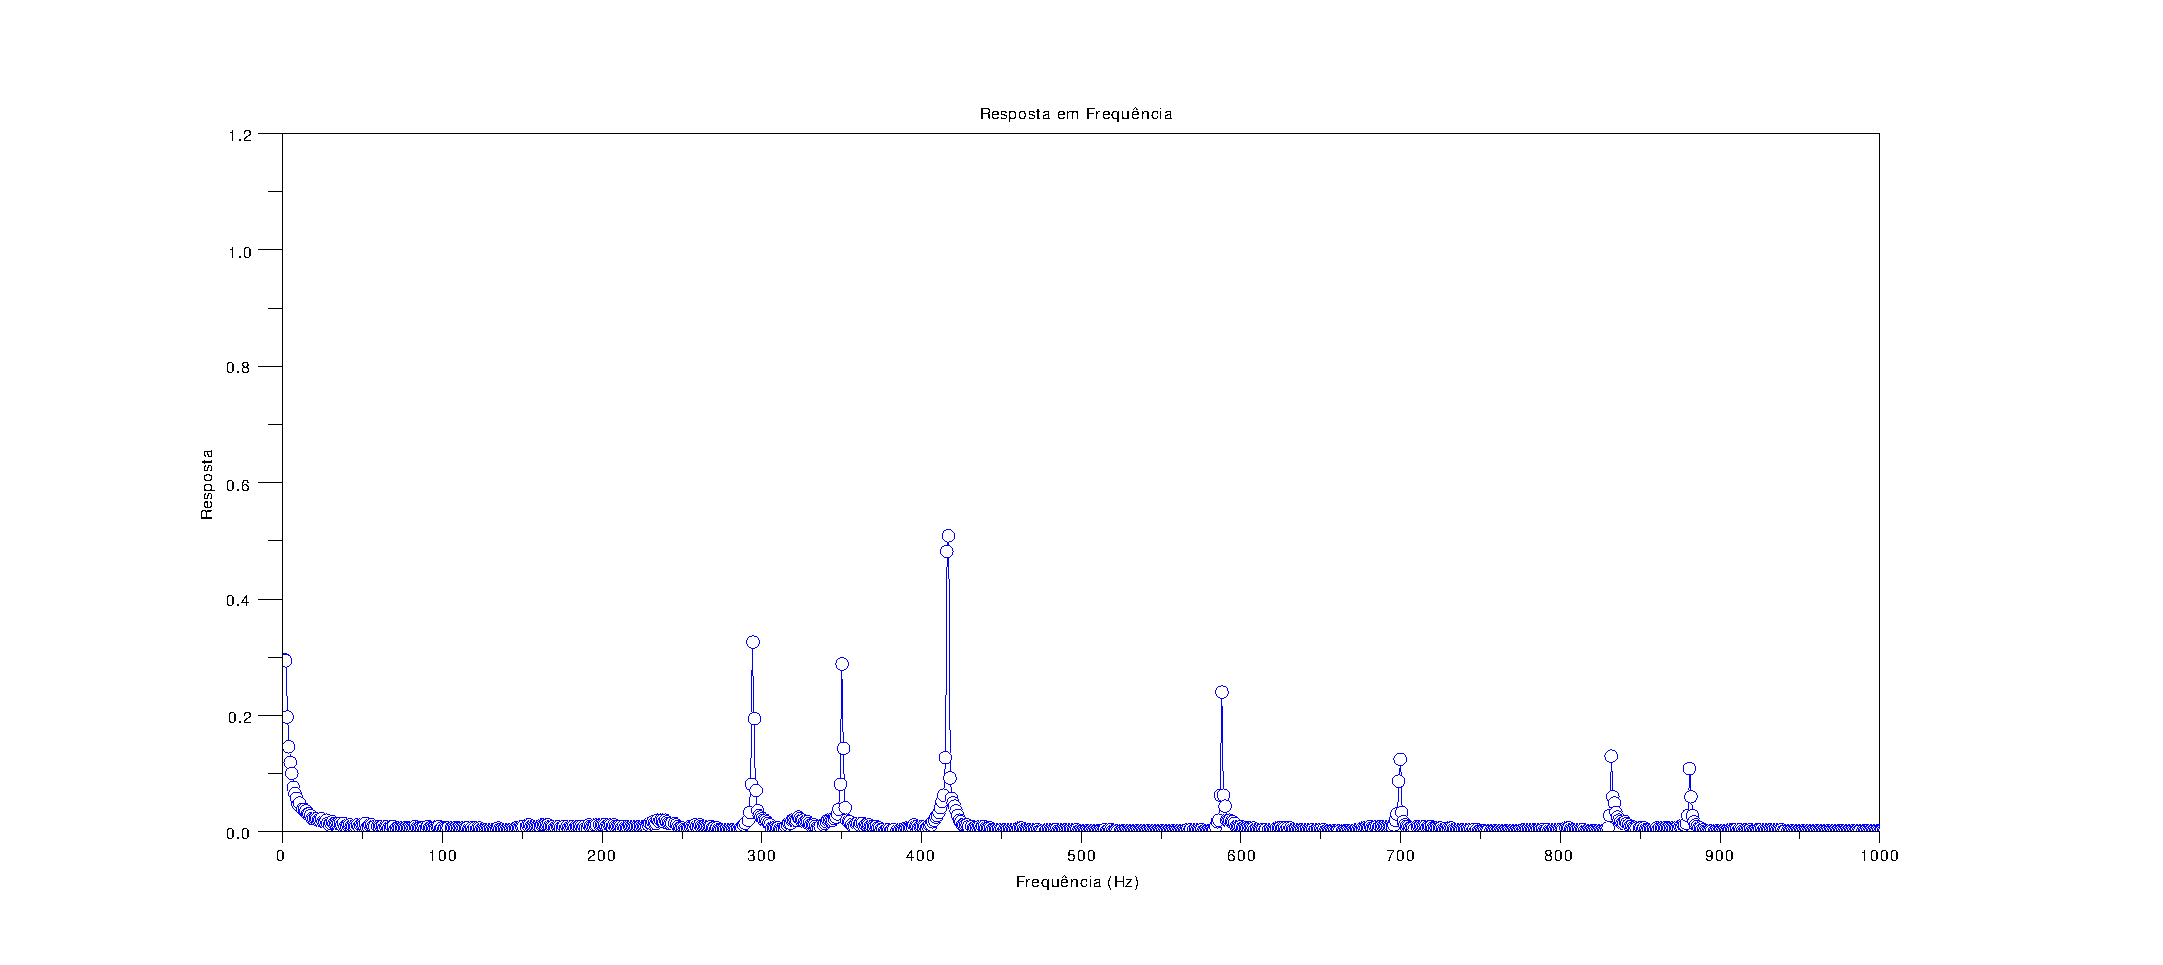
\includegraphics[keepaspectratio=true,scale=0.49]{figuras/Dm/fft_Ddim.eps}
	\caption{Gráfico da resposta em frequência para a gravação do acorde $Ddim$}
  \label{fig:espectro_Ddim}
\end{figure}

\begin{figure}[h]
	\centering
		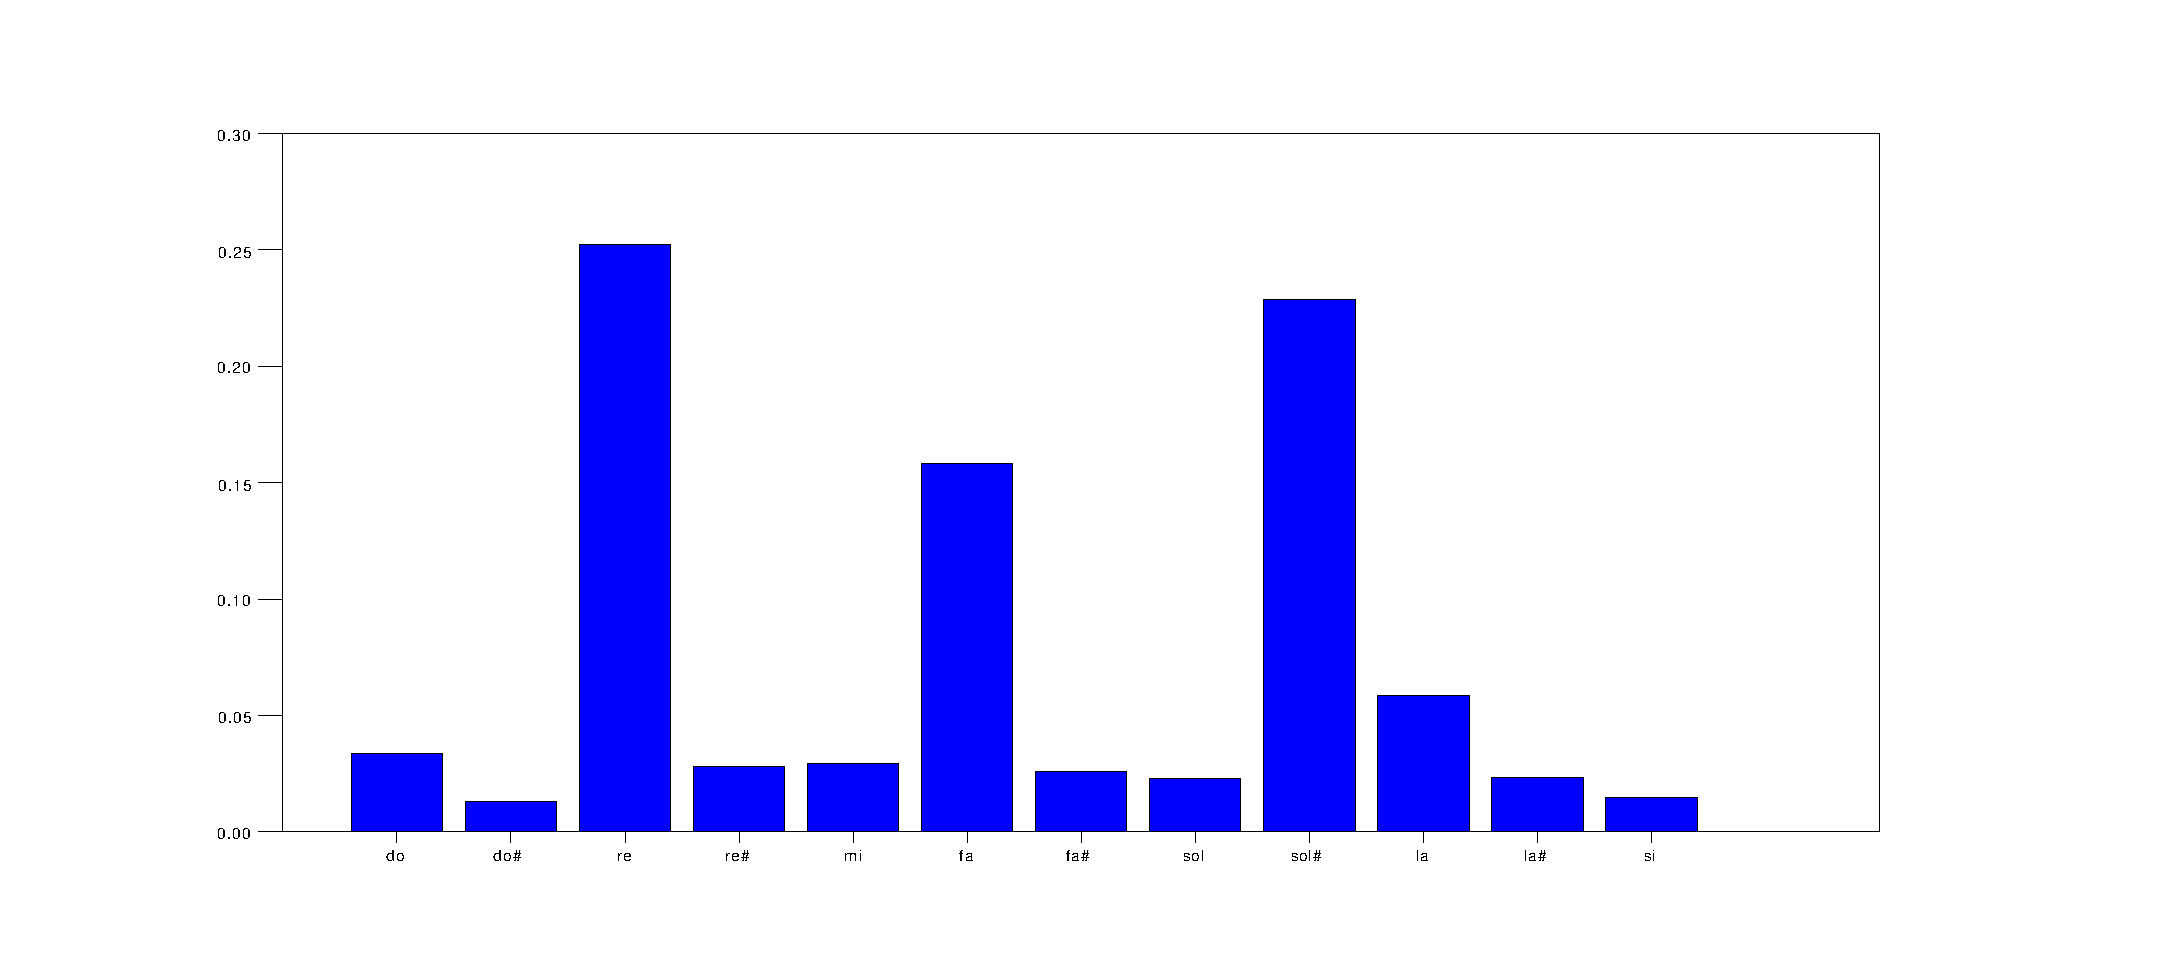
\includegraphics[keepaspectratio=true,scale=0.45]{figuras/Dm/notas_Ddim.eps}
	\caption{Gráfico de sugestão de notas para a gravação do acorde $Ddim$}
  \label{fig:notas_Ddim}
\end{figure}

\begin{figure}[h]
	\centering
		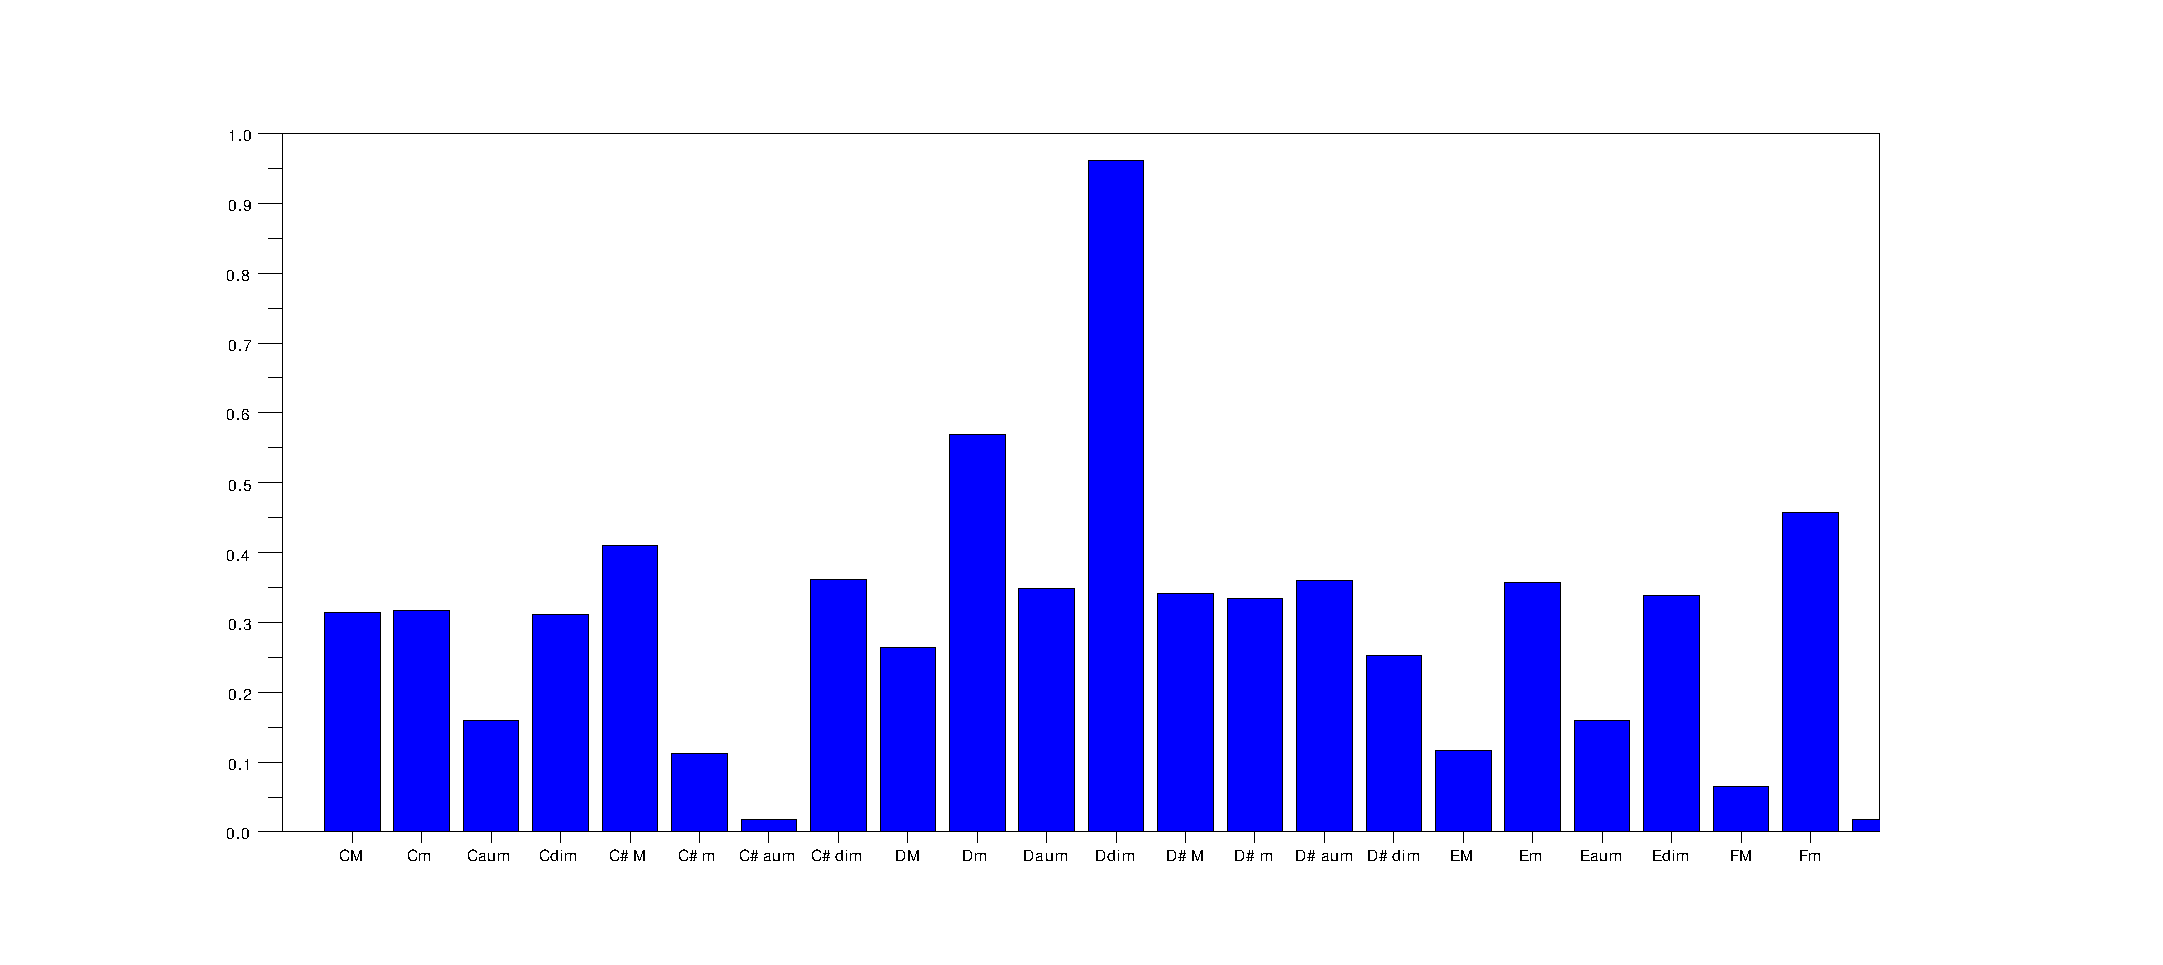
\includegraphics[keepaspectratio=true,scale=0.49]{figuras/Dm/acordes_1_Ddim.eps}
		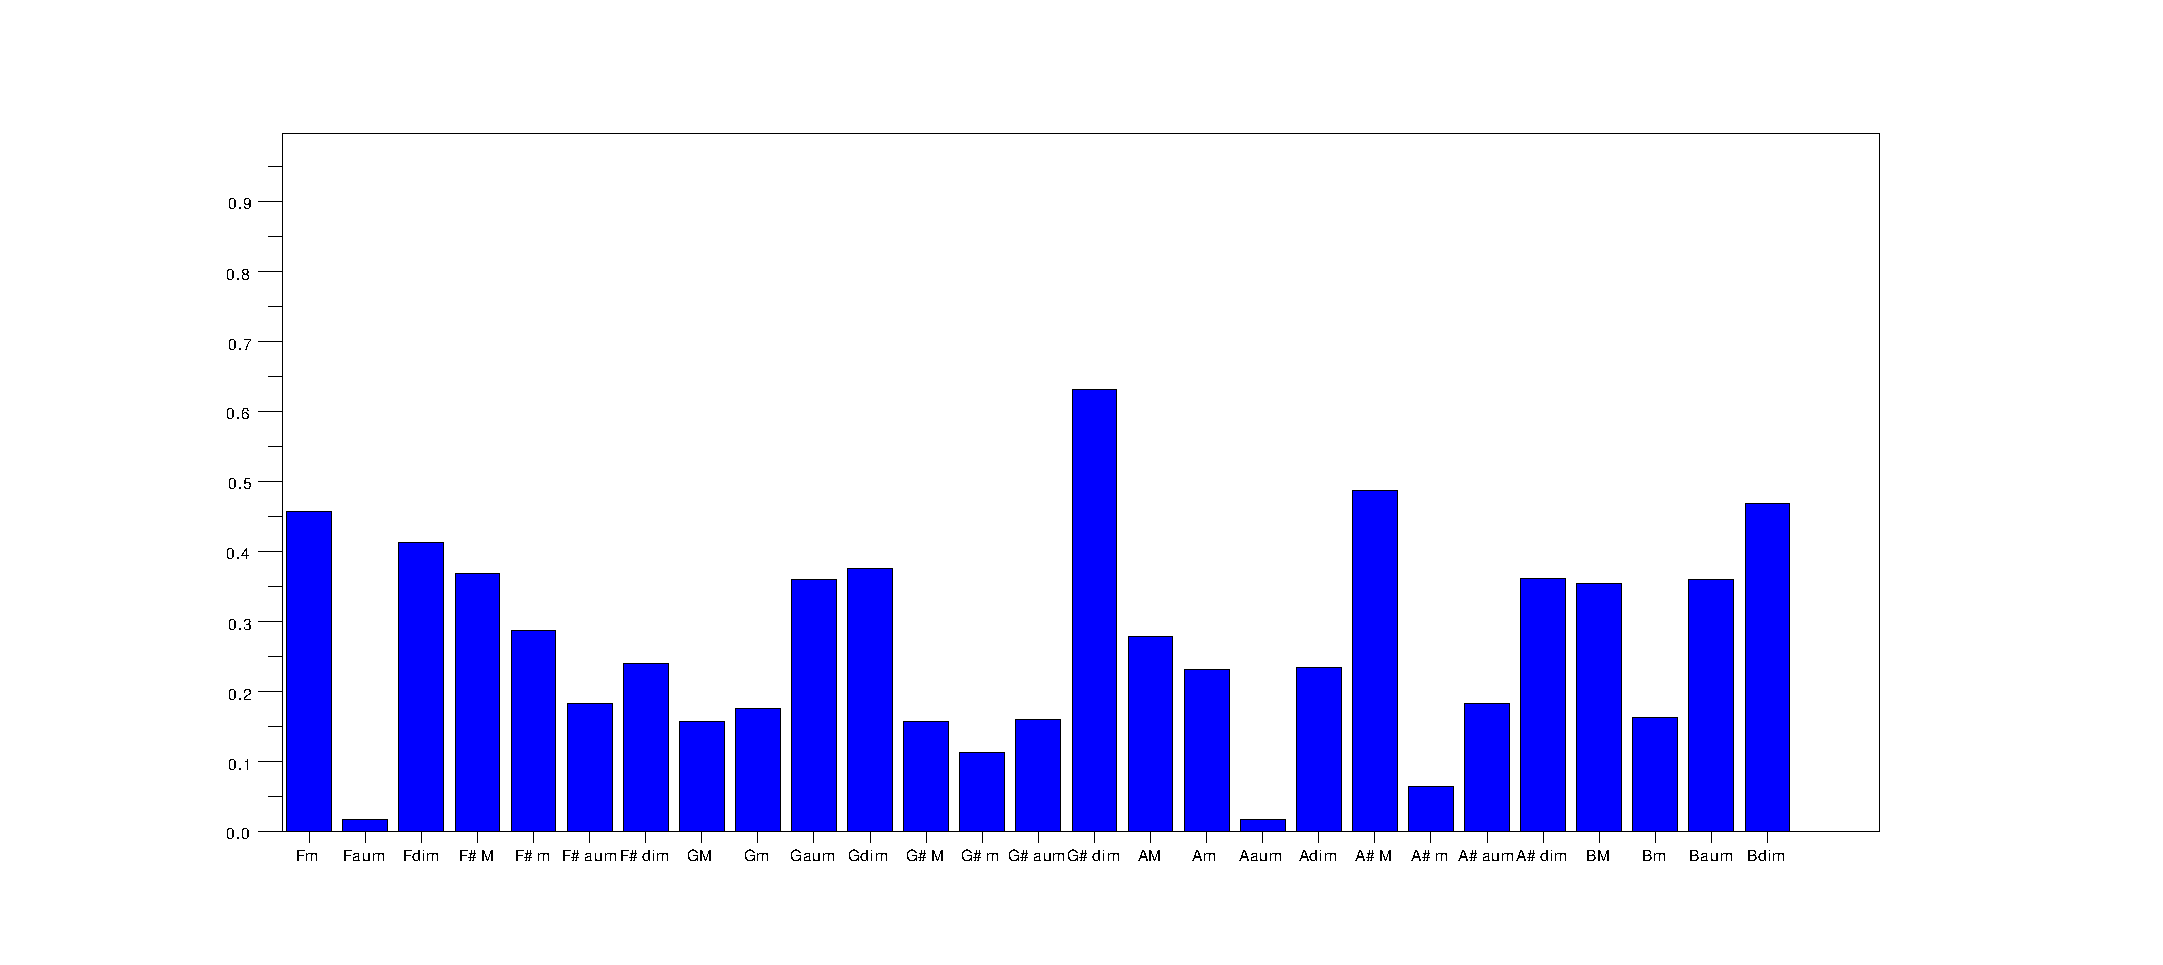
\includegraphics[keepaspectratio=true,scale=0.49]{figuras/Dm/acordes_2_Ddim.eps}
	\caption{Gráficos de sugestão de acordes a gravação do acorde $Ddim$}
  \label{fig:acordes_Ddim}
\end{figure}
\newpage

Do resultado da primeira camada de processamento é gerado o gráfico da figura \ref{fig:espectro_Ddim}. Esse gráfico diz respeito a natureza da composição do sinal em senoides em termos de transformada de fourier. O primeiro pico, no valor de 294 Hz, é relativo a nota $Ré$. O segundo pico, no valor de 350 Hz, é relativo a nota $Fá$. O terceiro pico, no valor de 417 Hz, é relativo a nota $Sol\#$. Os picos seguintes são relativos aos harmônicos dessas três notas.

Do resultado da segunda camada de processamento é gerado gráfico da figura \ref{fig:notas_Ddim}. É possível perceber nele que as notas $Ré$, $Fá$ e $Sol\#$ são as que mais possuem energia ou, no ponto de vista de sugestão, as mais sugeridas.

Do resultado da terceira camada de processamento são gerados os gráficos da figura \ref{fig:acordes_Ddim}. Essa camada é relativa ao resultados das sugestões de acordes musicais. É perceptível ver a presença da alta sugestão do acorde $Ddim$.

\subsection{Experimento 4 - Acorde $Daum$}
\label{sec:experimento4}

Nesse experimento foi tocado a tríade $Ré$ (baixo e tônica), $Fá\#$ e $Lá\#$ equivalente ao acorde $Daum$. A tríade foi tocada ao mesmo tempo e com a mesma força para todas as notas.

Segue os gráficos resultantes:

\begin{figure}[h]
	\centering
		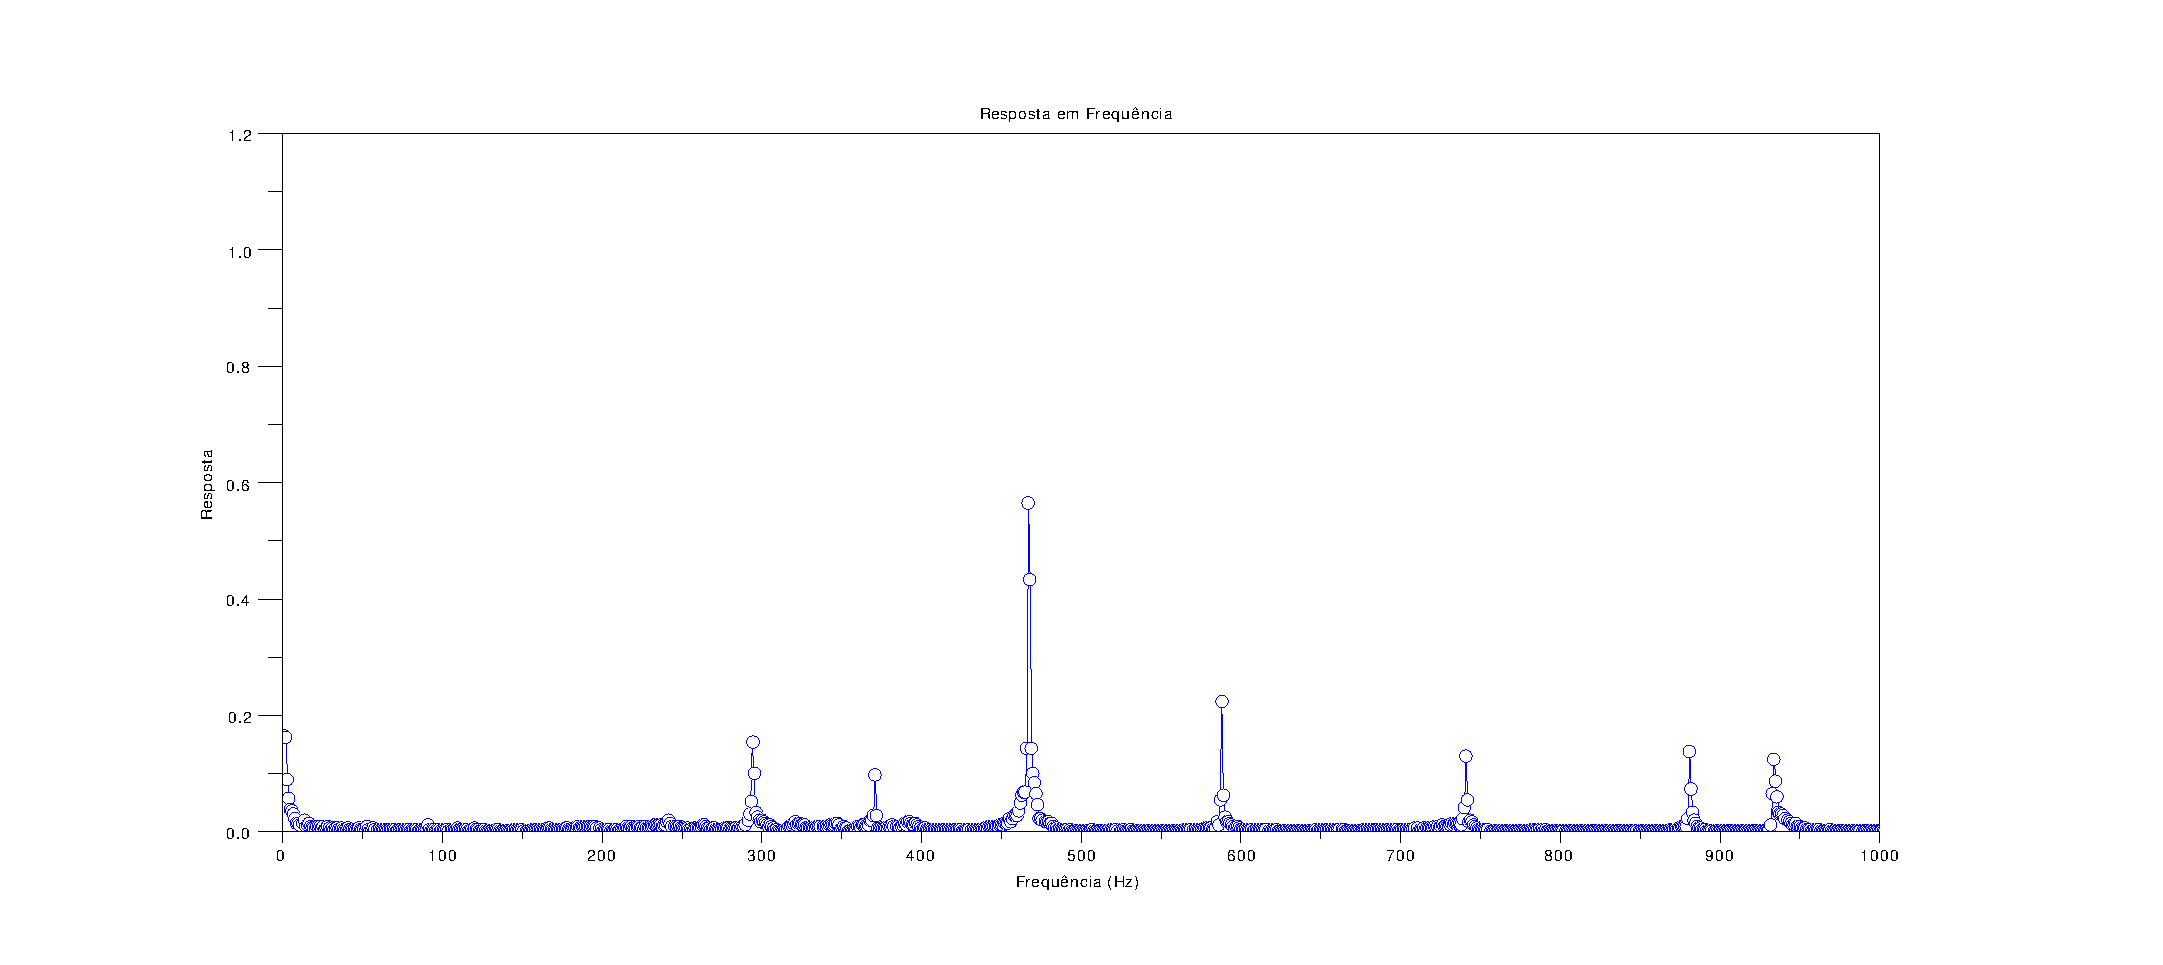
\includegraphics[keepaspectratio=true,scale=0.49]{figuras/Dm/fft_Daum.eps}
	\caption{Gráfico da resposta em frequência para a gravação do acorde $Daum$}
  \label{fig:espectro_Daum}
\end{figure}

\begin{figure}[h]
	\centering
		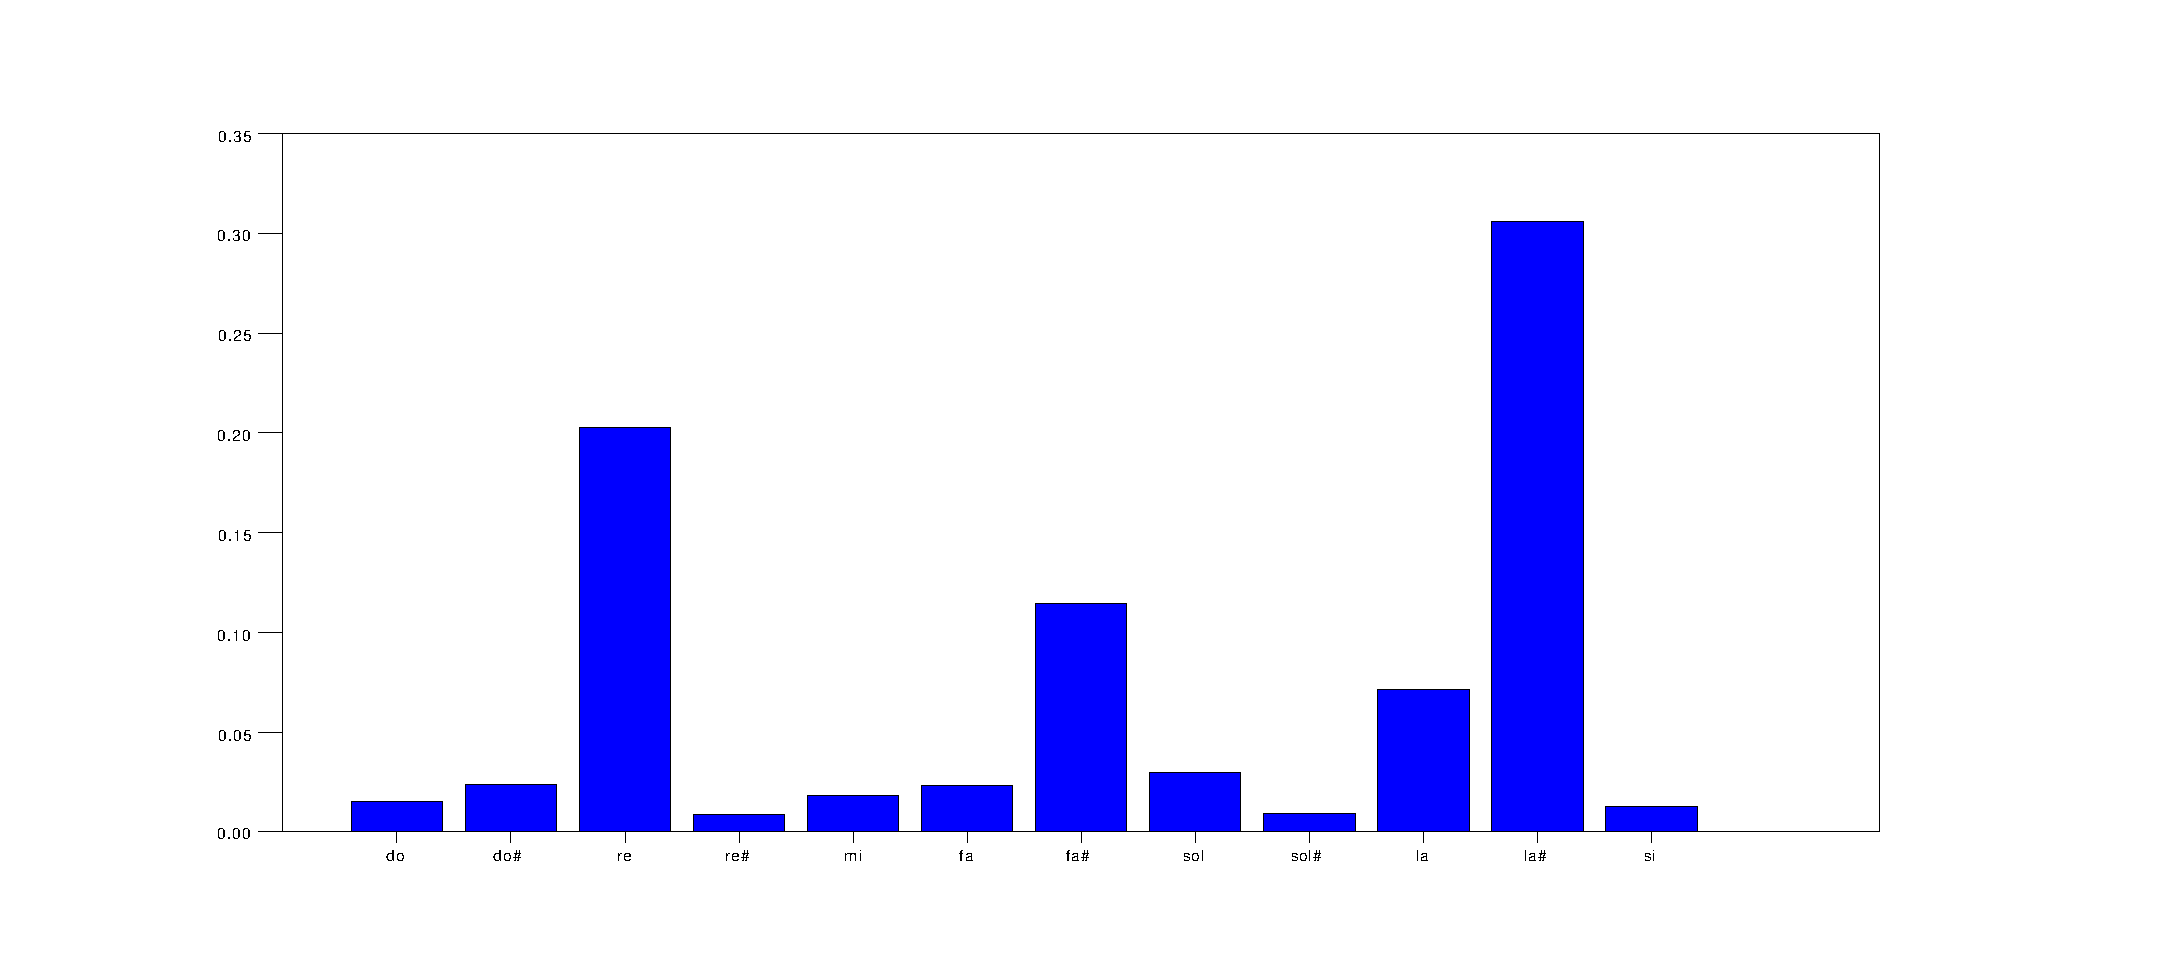
\includegraphics[keepaspectratio=true,scale=0.49]{figuras/Dm/notas_Daum.eps}
	\caption{Gráfico de sugestão de notas para a gravação do acorde $Daum$}
  \label{fig:notas_Daum}
\end{figure}

\begin{figure}[h]
	\centering
		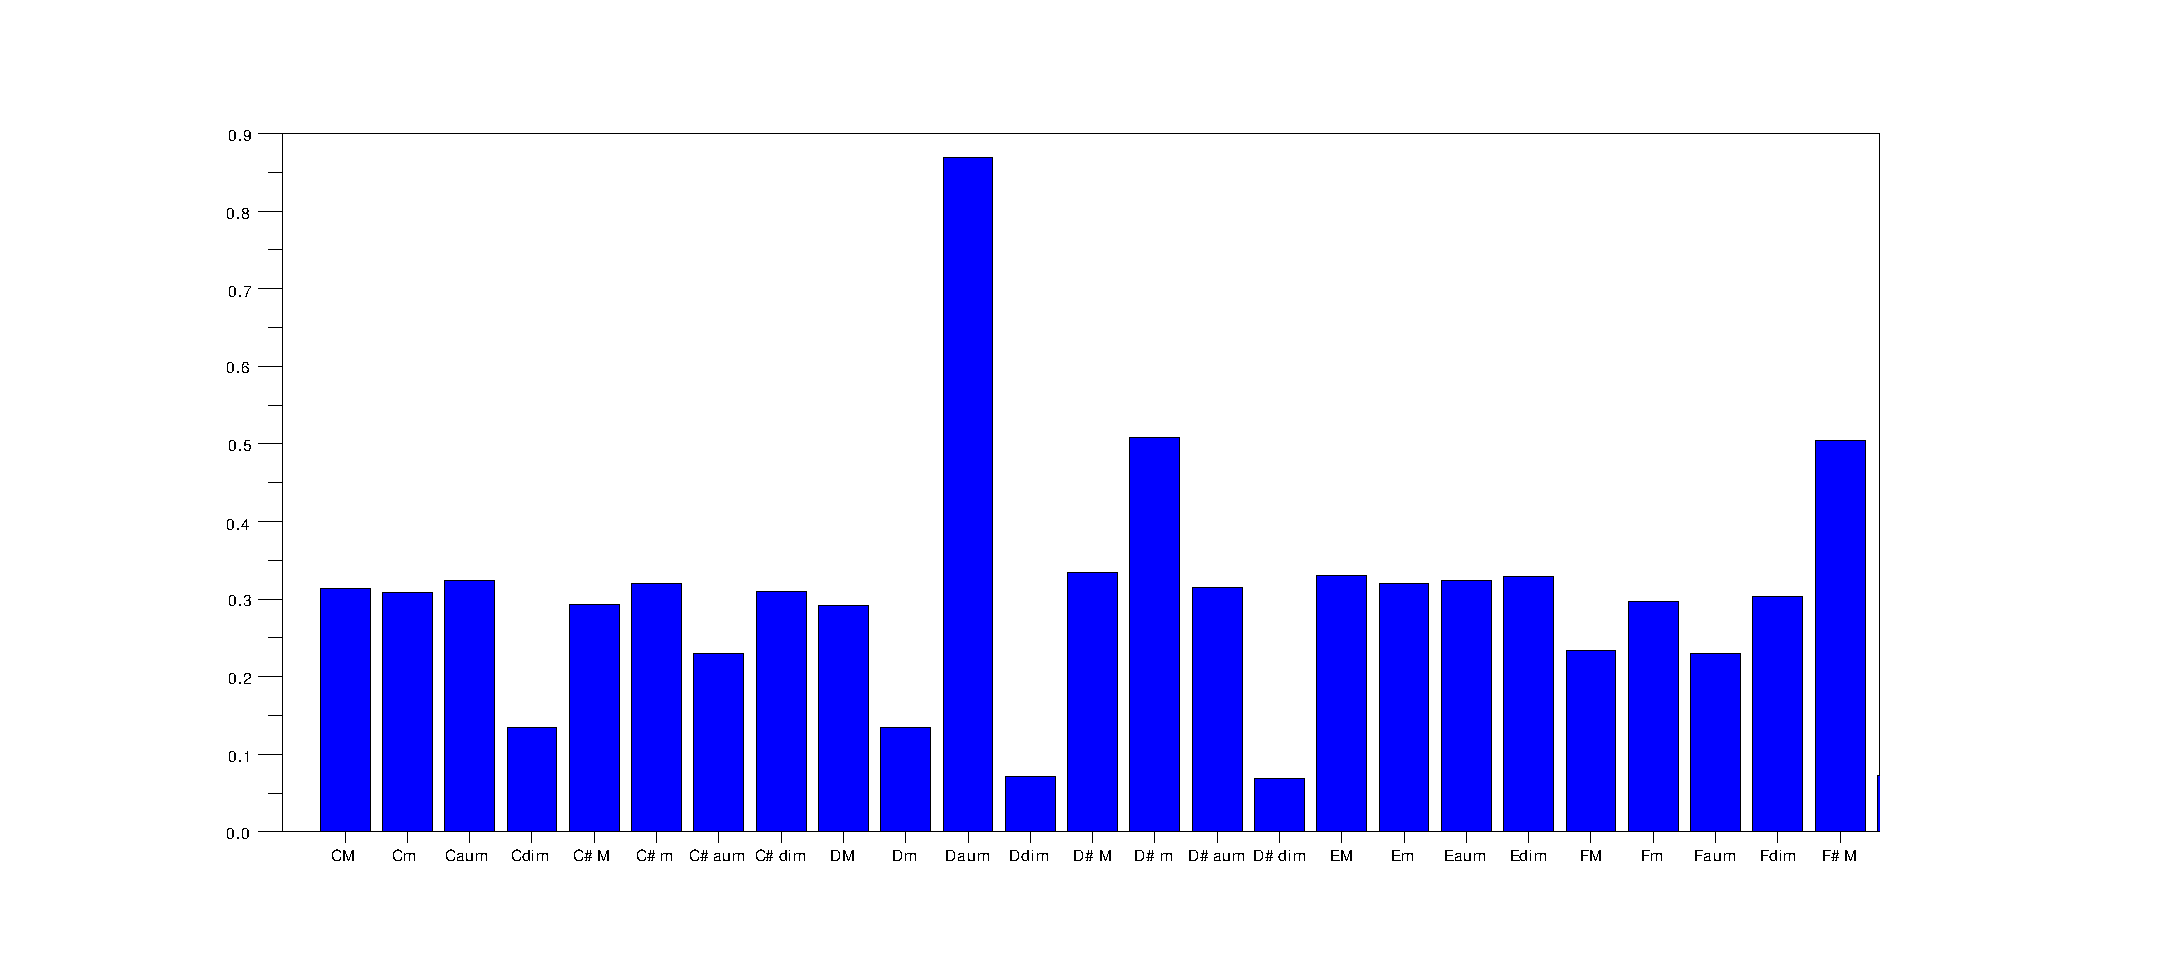
\includegraphics[keepaspectratio=true,scale=0.49]{figuras/Dm/acordes_1_Daum.eps}
		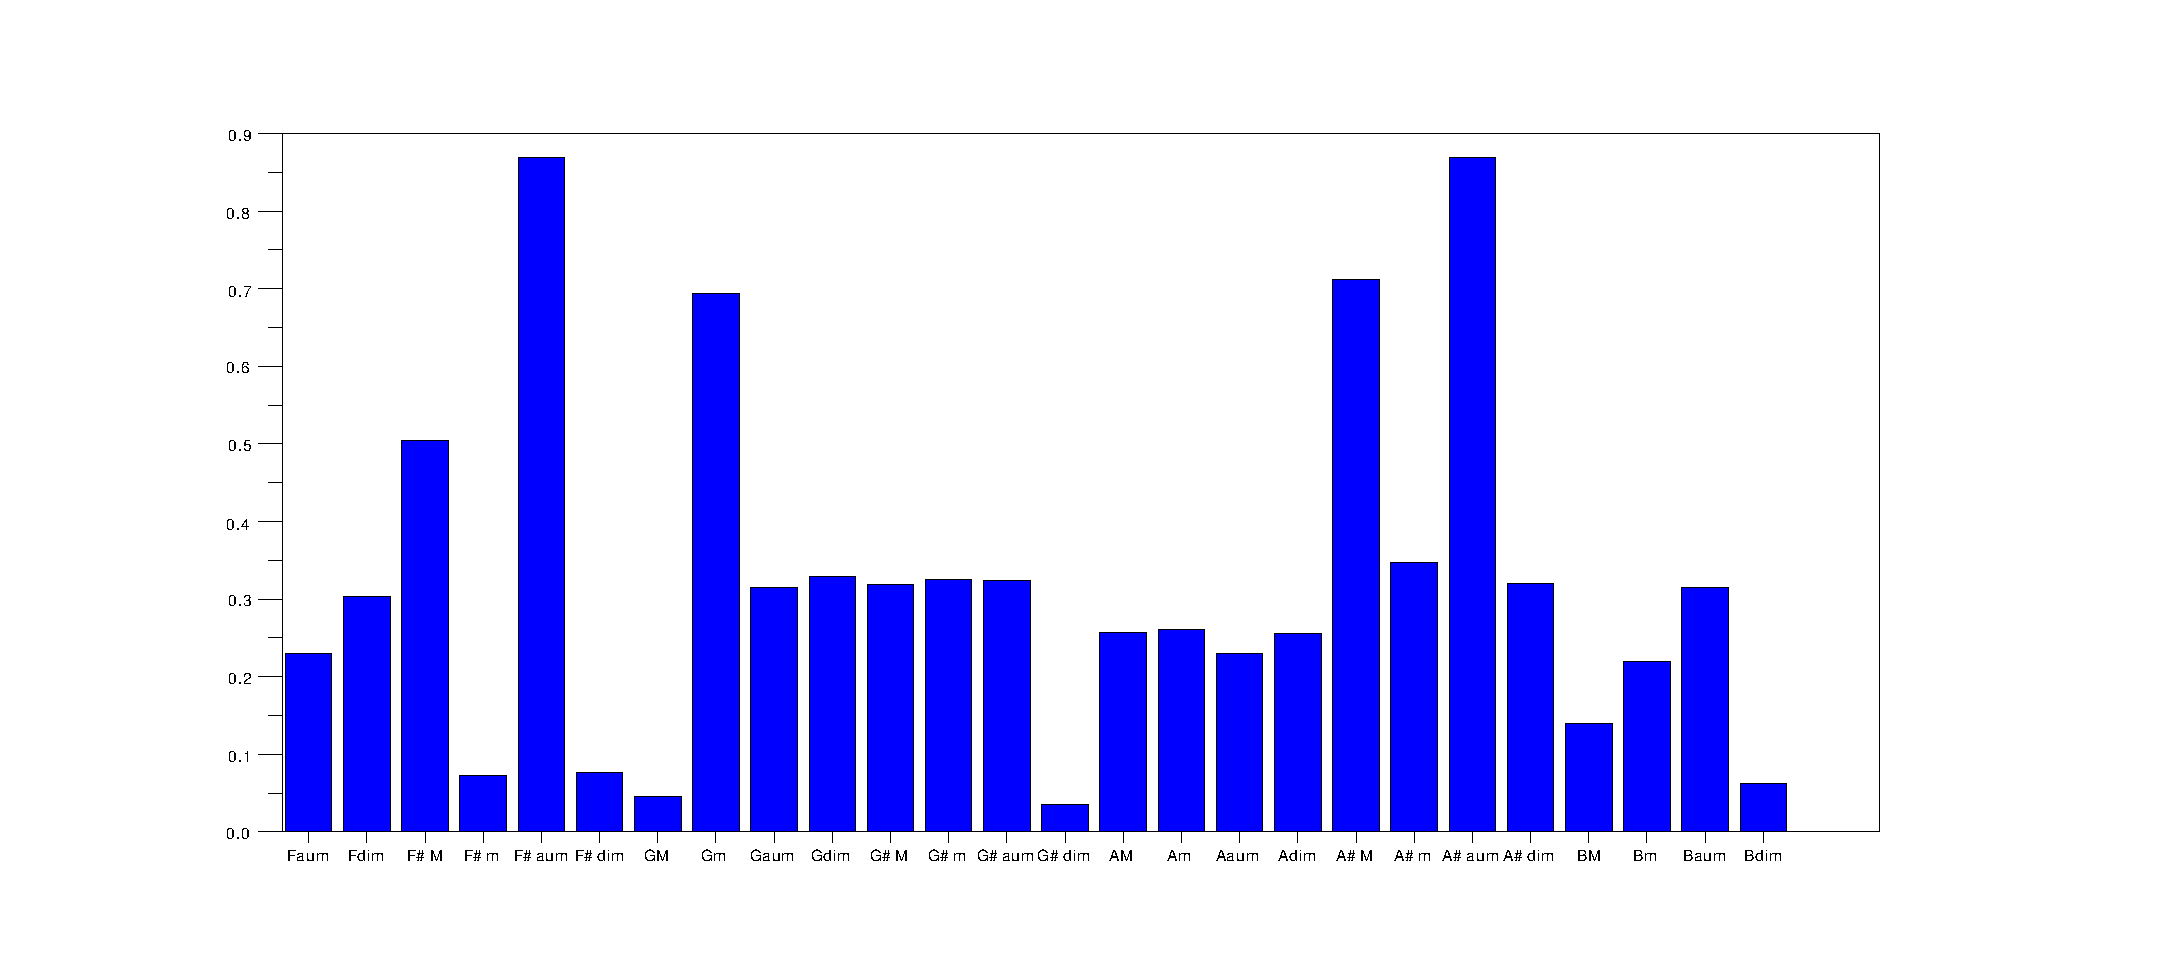
\includegraphics[keepaspectratio=true,scale=0.49]{figuras/Dm/acordes_2_Daum.eps}
	\caption{Gráficos de sugestão de acordes a gravação do acorde $Daum$}
  \label{fig:acordes_Daum}
\end{figure}
\newpage

Do resultado da primeira camada de processamento é gerado o gráfico da figura \ref{fig:espectro_Daum}. Esse gráfico diz respeito a natureza da composição do sinal em senoides em termos de transformada de fourier. O primeiro pico, no valor de 294 Hz, é relativo a nota $Ré$. O segundo pico, no valor de 371 Hz, é relativo a nota $Fá\#$. O terceiro pico, no valor de 467 Hz, é relativo a nota $Lá\#$. Os picos seguintes são relativos aos harmônicos dessas três notas.

Do resultado da segunda camada de processamento é gerado gráfico da figura \ref{fig:notas_Daum}. É possível perceber nele que as notas $Ré$, $Fá\#$ e $Lá\#$ são as que mais possuem energia ou, no ponto de vista de sugestão, as mais sugeridas.

Do resultado da terceira camada de processamento são gerados os gráficos da figura \ref{fig:acordes_Daum}. Essa camada é relativa aos resultados das sugestões de acordes musicais. É perceptível a alta sugestão dos acordes $Daum$, $F\#aum$ e $A\#aum$ com a mesma quantidade de energia. Isso é devido às notas comporem os mesmos acordes, diferenciando um do outro somente pela nota mais grave da tríade. Visto que o sistema possui o módulo de extração de baixos, a solução indicou que o acorde tocado foi $Daum$, visto que, como é mostrado no gráfico do espectro de frequências, a nota $Ré$ é a nota mais grave da tríade.

Segue na tabela \ref{tab:label_test} os resultados do sistema dado todas as combinações dos conjuntos de acordes de tríades possíveis. Esses resultados foram gerados pelo script disponível no repositório desse trabalho \footnote{https://github.com/josepedro/TCC}.

\begin{table}[ht!]
  %Vertical lines as column separators
  \centering
  \resizebox{0.9\textwidth}{!}{
  \begin{tabular}{ | c | c | c | c |}
    \hline
    - & \textbf{Acorde Fundamental} & \textbf{Quinta Invertida} & \textbf{Terça Invertida}\\
    \hline
    \textbf{C} & C & C/G & C/E \\
    \hline
    \textbf{Cm} & Cm & Cm/G & Cm/D\# \\
    \hline
    \textbf{Caum} & Caum & G\#aum & Eaum \\
    \hline
    \textbf{Cdim} & Cdim & Cdim/F\# & Cdim/D\# \\
    \hline
    \textbf{C\#} & C\# & C\#/G\# & C\#/F \\
    \hline
    \textbf{C\#m} & C\#m & C\#m/G\# & C\#m/E \\
    \hline
    \textbf{C\#aum} & C\#aum & Aaum & Faum \\
    \hline
    \textbf{C\#dim} & C\#dim & C\#dim/G & C\#dim/E \\
    \hline
    \textbf{D} & D & D/A & D/F\# \\
    \hline
    \textbf{Dm} & Dm & Dm/A & Dm/F \\
    \hline
    \textbf{Daum} & Daum & A\#aum & F\#aum \\
    \hline
    \textbf{Ddim} & Ddim & Ddim/G\# & Ddim/F \\
    \hline
    \textbf{D\#} & D\# & D\#/A\# & D\#/G \\
    \hline
    \textbf{D\#m} & D\#m & D\#m/A\# & D\#m/F\# \\
    \hline
    \textbf{D\#aum} & D\#aum & Baum & Gaum \\
    \hline
    \textbf{D\#dim} & D\#dim & D\#dim/A & D\#dim/F\# \\
    \hline
    \textbf{E} & E & E/B & E/G\# \\
    \hline
    \textbf{Em} & Em & Em/B & Em/G \\
    \hline
    \textbf{Eaum} & Eaum & Caum & G\#aum \\
    \hline
    \textbf{Edim} & Edim & Edim/A\# & Edim/G \\
    \hline
    \textbf{FM} & F & F/C & F/A \\
    \hline
    \textbf{Fm} & Fm & Fm/C & Fm/G\# \\
    \hline
    \textbf{Faum} & Faum & C\#aum & Aaum \\
    \hline
    \textbf{Fdim} & Fdim & Fdim/B & Fdim/G\# \\
    \hline
    \textbf{F\#} & F\# & F\#/C\# & F\#/A\# \\
    \hline
    \textbf{F\#m} & F\#m & F\#m/C\# & F\#m/A \\
    \hline
    \textbf{F\#aum} & F\#aum & Daum & A\#aum \\
    \hline
    \textbf{F\#dim} & F\#dim & F\#dim/C & F\#dim/A \\
    \hline
    \textbf{G} & G & G/D & G/B \\
    \hline
    \textbf{Gm} & Gm & Gm/D & Gm/A\# \\
    \hline
    \textbf{Gaum} & Gaum & D\#aum & Baum \\
    \hline
    \textbf{Gdim} & Gdim & Gdim/C\# & Gdim/A\# \\
    \hline
    \textbf{G\#} & G\# & G\#/D\# & G\#/C \\
    \hline
    \textbf{G\#m} & G\#m & G\#m/D\# & G\#m/B \\
    \hline
    \textbf{G\#aum} & G\#aum & Eaum & Caum \\
    \hline
    \textbf{G\#dim} & G\#dim & G\#dim/D & G\#dim/B \\
    \hline
    \textbf{A} & A & A/E & A/C\# \\
    \hline
    \textbf{Am} & Am & Am/E & Am/C \\
    \hline
    \textbf{Aaum} & Aaum & Faum & C\#aum \\
    \hline
    \textbf{Adim} & Adim & Adim/D\# & Adim/C \\
    \hline
    \textbf{A\#} & A\# & A\#/F & A\#/D \\
    \hline
    \textbf{A\#m} & A\#m & A\#m/F & A\#m/C\# \\
    \hline
    \textbf{A\#aum} & A\#aum & F\#aum & Daum \\
    \hline
    \textbf{A\#dim} & A\#dim & A\#dim/E & A\#dim/C\# \\
    \hline
    \textbf{B} & B & B/F\# & B/D\# \\
    \hline
    \textbf{Bm} & Bm & Bm/F\# & Bm/D \\
    \hline
    \textbf{Baum} & Baum & Gaum & D\#aum \\
    \hline
    \textbf{Bdim} & Bdim & Bdim/F & Bdim/D \\
    \hline
  \end{tabular}
  }
  \caption{Tabela de resultados dado os acordes tocados com inversões}
  \label{tab:label_test}
\end{table}

\section{Detecção de Transições Rítmicas}

\section{Implementação da Transformada Wavelets}

\section{Transcrição de Notas ao Longo do Tempo}

\section{Extração da Tonalidade do Áudio}

\section{Transcrição Automática de Acordes ao Longo do Tempo}